\documentclass[12pt,a4paper]{article}
\usepackage[utf8]{inputenc}
\usepackage[english]{babel}
\usepackage{geometry}
\usepackage{graphicx}
\usepackage{float}
\usepackage{placeins}
\usepackage{caption}
\usepackage{hyperref}
\usepackage{enumitem}
\usepackage{fancyhdr}
\usepackage{titlesec}
\usepackage{tocloft}
\usepackage{amsmath}
\usepackage{amsfonts}
\usepackage{amssymb}
\usepackage{textcomp} % or amssymb
% Page setup
\geometry{margin=1in}
\pagestyle{fancy}
\fancyhf{}
\fancyhead[L]{ENSIASD E-Learning Platform}
\fancyhead[R]{\thepage}
\renewcommand{\headrulewidth}{0.4pt}

% Title formatting
\titleformat{\section}{\Large\bfseries}{\thesection}{1em}{}
\titleformat{\subsection}{\large\bfseries}{\thesubsection}{1em}{}
\titleformat{\subsubsection}{\normalsize\bfseries}{\thesubsubsection}{1em}{}

% Hyperlink setup
\hypersetup{
    colorlinks=true,
    linkcolor=blue,
    filecolor=magenta,      
    urlcolor=cyan,
    pdftitle={ENSIASD E-Learning Platform Report},
    pdfauthor={ENSIASD Taroudant},
}

\begin{document}

% Title Page
\begin{titlepage}
    \centering
    \vspace*{2cm}
    
    {\Huge\bfseries ENSIASD E-Learning Platform}\\[0.5cm]
    {\Large Technical Documentation and Analysis Report}\\[2cm]
    
    {\large Prepared for}\\[0.3cm]
    {\Large\bfseries ENSIASD Taroudant}\\[2cm]
    
    {\large Document Version: 1.0}\\[0.5cm]
    {\large Date: \today}\\[3cm]
    
    \vfill
    
    {\large This report provides comprehensive documentation of the ENSIASD E-Learning Platform, including technical specifications, architecture analysis, and implementation details.}
    
\end{titlepage}

% Table of Contents
\tableofcontents
\newpage

\section{Introduction}

The ENSIASD E-Learning Platform represents a comprehensive digital educational solution tailored specifically for ENSIASD Taroudant, a prominent higher education institution. This report presents a detailed examination of the platform's architecture, functionality, and technical implementation, drawing from extensive analysis of the existing codebase, database structure, and system configuration.

ENSIASD Taroudant's E-Learning Platform emerges from the institution's commitment to educational innovation and digital transformation. At its core, the platform facilitates meaningful connections between instructors and students through technology, creating an environment where educational content delivery, student engagement, and administrative oversight converge seamlessly. The system recognizes that effective e-learning requires more than content delivery—it demands interaction, feedback, and community.

The platform serves three distinct user communities within ENSIASD Taroudant: students seeking flexible access to quality education, instructors requiring comprehensive tools for course delivery and student engagement, and administrators managing institutional content and system oversight.

This documentation encompasses both the technical foundations that power the platform and the user-centric features that define the learning experience. The analysis reveals a well-structured system that balances complexity with usability, offering robust functionality while maintaining the flexibility necessary for diverse educational scenarios. This report serves educators, administrators, and technical stakeholders who seek to understand the platform's capabilities and potential for enhancing the educational experience at ENSIASD Taroudant.

\subsection{Core Platform Capabilities}

\begin{itemize}
    \item \textbf{Dynamic Course Environment:} Instructors create rich, multi-layered courses featuring diverse content types, from traditional text and file resources to interactive quizzes and external learning materials.
    \item \textbf{Comprehensive Assessment Tools:} The platform supports varied assessment methods including assignments with flexible submission options, interactive quizzes, and detailed grading workflows with instructor feedback.
    \item \textbf{Collaborative Learning Spaces:} Course-specific discussion forums and announcement systems foster communication between instructors and students, creating virtual learning communities.
    \item \textbf{Institutional Web Presence:} A professionally designed public website showcases ENSIASD Taroudant's programs, mission, and educational offerings while providing prospective students with essential information.
    \item \textbf{Role-Based Access Management:} The platform implements sophisticated user role systems ensuring appropriate access levels:
    \begin{itemize}
        \item \textbf{Students:} Access course materials, submit assignments, participate in discussions, and track academic progress.
        \item \textbf{Instructors:} Design courses, manage content, assess student work, and facilitate learning experiences.
        \item \textbf{Administrators:} Oversee institutional content, manage public website elements, and maintain system-wide functionality.
    \end{itemize}
\end{itemize}

\section{Technical Architecture}

This section outlines the technical architecture and key components of the ENSIASD Taroudant E-Learning Platform.

\subsection{Backend Technologies}
\begin{itemize}
    \item \textbf{Framework:} Laravel 12 (PHP 8.2+)
    \item \textbf{Key Libraries:}
    \begin{itemize}
        \item \texttt{inertiajs/inertia-laravel}: For integrating the React frontend with the Laravel backend.
        \item \texttt{league/flysystem-aws-s3-v3}: For S3 file storage.
        \item \texttt{prism-php/prism}: Laravel package for integrating Large Language Models (LLMs).
        \item \texttt{tightenco/ziggy}: Enables usage of Laravel named routes in JavaScript.
    \end{itemize}
\end{itemize}

\subsection{Frontend Technologies}
\begin{itemize}
    \item \textbf{Framework/Library:} React 19 (using TypeScript)
    \item \textbf{Integration:} Inertia.js is used to build this single-page application (SPA) experience with server-side routing and controllers.
    \item \textbf{Key Libraries:}
    \begin{itemize}
        \item \texttt{@tiptap/react} \& Tiptap extensions: For a rich text editor experience.
        \item \texttt{@dnd-kit/core} \& \texttt{@dnd-kit/sortable}: For drag and drop functionality.
        \item \texttt{recharts}: For displaying charts (e.g., in instructor dashboards).
        \item \texttt{zod} \& \texttt{zod-form-data}: For schema validation.
        \item \texttt{date-fns}: For date utility functions.
        \item \texttt{sonner}: For toast notifications.
        \item \texttt{react-dropzone}: For file uploads.
        \item \texttt{cmdk}: Command menu component.
        \item \texttt{embla-carousel-react}: Carousel component.
        \item \texttt{framer-motion}: For animations.
    \end{itemize}
\end{itemize}

\subsection{Database Configuration}
\begin{itemize}
    \item \textbf{Default (Development):} SQLite (as configured in \texttt{config/database.php} and \texttt{composer.json} post-install script).
    \item \textbf{Supported Production Databases:} MySQL, PostgreSQL, MariaDB, SQL Server (as listed in \texttt{config/database.php}).
    \item \textbf{Caching:} Redis is also configured for caching and potentially other uses.
\end{itemize}

\subsection{Styling and UI Components}
\begin{itemize}
    \item \textbf{CSS Framework:} Tailwind CSS (Version 4).
    \item \textbf{UI Components:} The project heavily utilizes Radix UI primitive components (e.g., \texttt{@radix-ui/react-accordion}, \texttt{@radix-ui/react-dialog}, etc.) and Lucide Icons (\texttt{lucide-react}). This component structure, found under \texttt{resources/js/components/ui}, is characteristic of component libraries like Shadcn UI, which are built on these primitives.
    \item \textbf{Utility Libraries:} \texttt{class-variance-authority}, \texttt{clsx}, \texttt{tailwind-merge} for managing CSS classes.
    \item \textbf{Animations:} \texttt{tailwindcss-animate}.
\end{itemize}

\subsection{API and Routing}
\begin{itemize}
    \item The application primarily functions as a web application using server-side rendering via Inertia.js.
    \item There is no dedicated \texttt{routes/api.php} file for token-based API routes. Specific interactions, such as quiz generation (\texttt{POST /quiz/generate}), are handled via web routes defined in \texttt{routes/web.php}, likely as AJAX requests within the authenticated session.
\end{itemize}

\subsection{Development Tools}
\begin{itemize}
    \item \textbf{Build Tool:} Vite: Used for frontend asset bundling and development server, configured in \texttt{vite.config.mjs}.
    \item \textbf{Version Control:} Git: Inferred from the presence of \texttt{.git} related files and common development practices.
    \item \textbf{Server Environment (General Assumption):} A standard PHP server environment, such as Nginx or Apache with PHP-FPM, is required to host the Laravel backend. A Node.js environment is necessary for the frontend build process.
\end{itemize}

\section{User Roles and Functionality}

The platform's effectiveness stems from its careful attention to the distinct needs of each user type within the educational ecosystem. Rather than adopting a one-size-fits-all approach, the system provides tailored experiences that enhance productivity and engagement for students, instructors, and administrators alike.

\subsection{User Roles}

The platform defines three primary user roles, each with specific capabilities:

\begin{itemize}
    \item \textbf{Student:}
    \begin{itemize}
        \item \textbf{Course Interaction:} Enrolls in available courses using course codes or invite links. Accesses all published course materials, including chapters, uploaded resources (documents, videos, links), and embedded rich text content.
        \item \textbf{Assignments \& Quizzes:} Submits assignments as per instructor requirements (potentially including text and file uploads). Takes quizzes designed to assess understanding of course content.
        \item \textbf{Communication:} Participates in course-specific discussion forums by creating new threads or commenting on existing ones. Views course announcements made by instructors and can comment on them.
        \item \textbf{Progress \& Profile:} Tracks their progress and grades for assignments and quizzes (implied by submission and grading features). Manages their personal profile information (name, avatar, etc.).
    \end{itemize}
    \item \textbf{Instructor:}
    \begin{itemize}
        \item \textbf{Course Management:} Creates new courses, providing details such as title, description, image, category, and a unique color theme. Organizes courses into reorderable chapters. Adds and manages diverse learning resources within chapters (rich text, file attachments, external web links). Controls course status (draft, published, archived).
        \item \textbf{Assessment Management:} Creates, edits, and manages assignments with detailed instructions, due dates, and optional attachments. Develops and administers quizzes with various question types and options.
        \item \textbf{Student Interaction \& Grading:} Views student submissions for assignments. Provides grades and textual feedback on submissions.
        \item \textbf{Communication \& Engagement:} Posts course-specific announcements to students, which can include content and attachments. Manages and participates in course discussion forums.
        \item \textbf{Enrollment Management:} Manages student enrollments within their courses, including the ability to remove students if necessary.
        \item \textbf{Dashboard \& Analytics:} Accesses a dedicated dashboard providing statistics on their courses, such as total student numbers, active student counts, enrollment trends over time, and distribution of resource types used.
        \item \textbf{Profile Management:} Manages their personal and professional profile information.
    \end{itemize}
    \item \textbf{Administrator:}
    \begin{itemize}
        \item \textbf{Public Website Content Management:} Manages the content of the public-facing website pages, including the Home page (e.g., hero section text, images, links), About page (mission, vision, features, stats), Contact page (contact details, map), and Publications/Announcements page. This is managed through a dedicated interface in the backend.
    \end{itemize}
\end{itemize}

\subsection{Platform Features}

Beyond role-specific capabilities, the platform integrates numerous features that work together to create a cohesive educational environment. These features address the fundamental requirements of modern e-learning while providing flexibility for diverse teaching and learning styles:

\begin{itemize}
    \item \textbf{User Authentication \& Authorization:}
    \begin{itemize}
        \item Secure user registration and login mechanisms.
        \item Password management (e.g., reset functionality).
        \item Role-based access control, ensuring users only access features relevant to their role.
        \item A profile completion step for new users to ensure necessary information is provided.
    \end{itemize}
    \item \textbf{Course Creation \& Management:}
    \begin{itemize}
        \item Instructors can create courses with comprehensive details: title, description, cover image, category, display color, and status (draft, published, archived).
        \item Automatic generation of unique course codes and shareable invite tokens for easy student enrollment.
        \item Courses can be structured into logical chapters, which instructors can reorder as needed.
        \item A variety of resource types can be added to chapters:
        \begin{itemize}
            \item \textbf{Rich Text:} For creating formatted textual content directly on the platform.
            \item \textbf{Attachments:} For uploading files (documents, presentations, media).
            \item \textbf{External Links:} For linking to external web resources.
        \end{itemize}
    \end{itemize}
    \item \textbf{Assignment Management:}
    \begin{itemize}
        \item Instructors can create assignments with titles, detailed instructions, specific due dates, and attach relevant files.
        \item Control over assignment visibility through a publish/unpublish mechanism.
    \end{itemize}
    \item \textbf{Submission System:}
    \begin{itemize}
        \item Students can submit their work for assignments, typically involving text input and/or file uploads.
        \item Instructors have an interface to view all submissions for an assignment, access submitted files, and assign grades and provide written feedback.
    \end{itemize}
    \item \textbf{Quiz System:}
    \begin{itemize}
        \item Includes functionality for generating quizzes (\texttt{QuizController::generateQuiz}).
        \item Supports the creation of quiz questions, multiple-choice options (or other question types), and tracks student answers. This allows for automated or instructor-led assessment of learning.
    \end{itemize}
    \item \textbf{Announcement System:}
    \begin{itemize}
        \item Instructors can create and post announcements visible to all students within a specific course.
        \item Announcements can contain formatted text and include file attachments.
        \item A commenting feature allows for interaction and clarification on announcements.
    \end{itemize}
    \item \textbf{Discussion Forum:}
    \begin{itemize}
        \item Each course has its own dedicated discussion forum.
        \item Students and instructors can create new discussion threads on relevant topics.
        \item Users can post comments within threads, fostering a collaborative learning environment.
    \end{itemize}
    \item \textbf{Instructor Dashboard:}
    \begin{itemize}
        \item A personalized dashboard for instructors provides key statistics and insights into their courses and student engagement. This includes:
        \begin{itemize}
            \item Aggregate counts: total students, number of courses.
            \item Activity metrics: currently active students.
            \item Growth indicators: percentage changes in student numbers and course creation.
            \item Visualizations: Charts displaying enrollment trends over time and a breakdown of resource types used across courses.
        \end{itemize}
    \end{itemize}
    \item \textbf{Public Website \& Content Management:}
    \begin{itemize}
        \item The platform includes a public-facing website with several key pages:
        \begin{itemize}
            \item \textbf{Home:} Landing page with introductory content, featured courses, and platform highlights.
            \item \textbf{About:} Information about ENSIASD Taroudant and the e-learning platform's mission and features.
            \item \textbf{Courses:} A public listing of available courses, potentially with search and filtering capabilities by category.
            \item \textbf{Publications:} A section for general announcements, news, or articles from the institution.
            \item \textbf{Contact:} Contact information and a contact form or map.
        \end{itemize}
        \item The content for these public pages is dynamically manageable by an Administrator via a backend interface, allowing updates to text, images, and other elements without code changes.
    \end{itemize}
    \item \textbf{Profile Management:}
    \begin{itemize}
        \item All users (Students, Instructors, Administrators) can manage their personal profile information, including name, email, password, and avatar.
    \end{itemize}
    \end{itemize}
\end{itemize}

\section{Database Architecture and Data Modeling}

The platform's data architecture reflects the complex relationships inherent in educational environments. The database design accommodates diverse content types, user interactions, and assessment methods while maintaining referential integrity and supporting efficient queries. The following entities form the foundation of the platform's data model:

\subsection{Core Database Entities}

\begin{itemize}
    \item \textbf{User (\texttt{users} table):}
    \begin{itemize}
        \item \textbf{Attributes:} \texttt{id} (PK), \texttt{name}, \texttt{username}, \texttt{email} (unique), \texttt{avatar}, \texttt{role} (e.g., student, instructor, admin), \texttt{profile\_completed\_at} (timestamp), \texttt{password}, \texttt{email\_verified\_at} (timestamp), \texttt{remember\_token}, \texttt{created\_at}, \texttt{updated\_at}.
        \item \textbf{Relationships:}
        \begin{itemize}
            \item \texttt{InstructorProfile}: One-to-One (User has one InstructorProfile). Foreign Key: \texttt{instructor\_profiles.user\_id}.
            \item \texttt{CourseEnrollment}: One-to-Many (User has many CourseEnrollments). Foreign Key: \texttt{course\_enrollments.user\_id}.
            \item \texttt{Course} (as instructor): One-to-Many (User (instructor) has many Courses). Foreign Key: \texttt{courses.instructor\_id}.
            \item \texttt{CourseThread} (as author): One-to-Many (User has many CourseThreads). Foreign Key: \texttt{course\_threads.author\_id}.
            \item \texttt{ThreadComment} (as author): One-to-Many (User has many ThreadComments). Foreign Key: \texttt{thread\_comments.author\_id}.
            \item \texttt{Submission}: One-to-Many (User has many Submissions). Foreign Key: \texttt{submissions.user\_id}.
            \item \texttt{Announcement} (as author): One-to-Many (User has many Announcements). Foreign Key: \texttt{announcements.user\_id}.
            \item \texttt{AnnouncementComment} (as author): One-to-Many (User has many AnnouncementComments). Foreign Key: \texttt{announcement\_comments.user\_id}.
            \item \texttt{courses} (as student): Many-to-Many via \texttt{CourseEnrollment} (User belongs to many Courses).
        \end{itemize}
    \end{itemize}
    \item \textbf{InstructorProfile (\texttt{instructor\_profiles} table):}
    \begin{itemize}
        \item \textbf{Attributes:} \texttt{id} (PK), \texttt{user\_id} (FK to \texttt{users.id}), \texttt{bio}, \texttt{expertise\_areas} (array/JSON), \texttt{social\_links} (array/JSON), \texttt{created\_at}, \texttt{updated\_at}.
        \item \textbf{Relationships:}
        \begin{itemize}
            \item \texttt{User}: One-to-One (InstructorProfile belongs to one User).
        \end{itemize}
    \end{itemize}
    \item \textbf{Course (\texttt{courses} table):}
    \begin{itemize}
        \item \textbf{Attributes:} \texttt{id} (PK), \texttt{instructor\_id} (FK to \texttt{users.id}), \texttt{title}, \texttt{description}, \texttt{image} (path/URL), \texttt{code} (unique course code), \texttt{invite\_token} (unique for link-based enrollment), \texttt{color}, \texttt{category}, \texttt{status} (enum: draft, published, archived), \texttt{published\_at} (timestamp), \texttt{created\_at}, \texttt{updated\_at}.
        \item \textbf{Relationships:}
        \begin{itemize}
            \item \texttt{User} (instructor): Many-to-One (Course belongs to one User (instructor)).
            \item \texttt{Chapter}: One-to-Many (Course has many Chapters). Foreign Key: \texttt{chapters.course\_id}.
            \item \texttt{CourseEnrollment}: One-to-Many (Course has many CourseEnrollments). Foreign Key: \texttt{course\_enrollments.course\_id}.
            \item \texttt{CourseThread}: One-to-Many (Course has many CourseThreads). Foreign Key: \texttt{course\_threads.course\_id}.
            \item \texttt{Announcement}: One-to-Many (Course has many Announcements). Foreign Key: \texttt{announcements.course\_id}.
            \item \texttt{Assignment}: One-to-Many (Course has many Assignments). Foreign Key: \texttt{assignments.course\_id}.
            \item \texttt{students} (Users): Many-to-Many via \texttt{CourseEnrollment} (Course has many Students).
        \end{itemize}
    \end{itemize}
    \item \textbf{Chapter (\texttt{chapters} table):}
    \begin{itemize}
        \item \textbf{Attributes:} \texttt{id} (PK), \texttt{course\_id} (FK to \texttt{courses.id}), \texttt{title}, \texttt{description}, \texttt{position} (integer for ordering), \texttt{created\_at}, \texttt{updated\_at}.
        \item \textbf{Relationships:}
        \begin{itemize}
            \item \texttt{Course}: Many-to-One (Chapter belongs to one Course).
            \item \texttt{Resource}: One-to-Many (Chapter has many Resources). Foreign Key: \texttt{resources.chapter\_id}.
        \end{itemize}
    \end{itemize}
    \item \textbf{Resource (\texttt{resources} table):} (Central table for typed resources)
    \begin{itemize}
        \item \textbf{Attributes:} \texttt{id} (PK), \texttt{chapter\_id} (FK to \texttt{chapters.id}), \texttt{title}, \texttt{resource\_type} (enum: 'rich\_text', 'attachment\_collection', 'external\_link', 'quiz'), \texttt{position} (integer for ordering), \texttt{metadata} (JSON), \texttt{created\_at}, \texttt{updated\_at}.
        \item \textbf{Relationships:}
        \begin{itemize}
            \item \texttt{Chapter}: Many-to-One (Resource belongs to one Chapter).
            \item \texttt{RichTextResource}: One-to-One. Foreign Key: \texttt{rich\_text\_resources.resource\_id}.
            \item \texttt{AttachmentResource}: One-to-One (representing a collection of attachments for this resource). Foreign Key: \texttt{attachment\_resources.resource\_id}.
            \item \texttt{ExternalResource}: One-to-One. Foreign Key: \texttt{external\_resources.resource\_id}.
            \item \texttt{QuizQuestion}: One-to-Many (A 'quiz' type Resource can have many QuizQuestions). Foreign Key: \texttt{quiz\_questions.resource\_id}.
        \end{itemize}
    \end{itemize}
    \item \textbf{RichTextResource (\texttt{rich\_text\_resources} table):}
    \begin{itemize}
        \item \textbf{Attributes:} \texttt{id} (PK), \texttt{resource\_id} (FK to \texttt{resources.id}), \texttt{content} (text/HTML), \texttt{format} (e.g., 'html', 'markdown'), \texttt{created\_at}, \texttt{updated\_at}.
        \item \textbf{Relationships:}
        \begin{itemize}
            \item \texttt{Resource}: One-to-One (RichTextResource belongs to one Resource).
        \end{itemize}
    \end{itemize}
    \item \textbf{AttachmentResource (\texttt{attachment\_resources} table):} (Represents a resource that is a collection of files)
    \begin{itemize}
        \item \textbf{Attributes:} \texttt{id} (PK), \texttt{resource\_id} (FK to \texttt{resources.id}), \texttt{created\_at}, \texttt{updated\_at}.
        \item \textbf{Relationships:}
        \begin{itemize}
            \item \texttt{Resource}: One-to-One (AttachmentResource belongs to one Resource).
            \item \texttt{Attachment}: Polymorphic One-to-Many (AttachmentResource can have many Attachments). \texttt{attachable\_id} \& \texttt{attachable\_type} on \texttt{attachments} table.
        \end{itemize}
    \end{itemize}
    \item \textbf{ExternalResource (\texttt{external\_resources} table):}
    \begin{itemize}
        \item \textbf{Attributes:} \texttt{id} (PK), \texttt{resource\_id} (FK to \texttt{resources.id}), \texttt{external\_url}, \texttt{link\_title}, \texttt{link\_description}, \texttt{favicon\_url}, \texttt{og\_image\_url}, \texttt{created\_at}, \texttt{updated\_at}.
        \item \textbf{Relationships:}
        \begin{itemize}
            \item \texttt{Resource}: One-to-One (ExternalResource belongs to one Resource).
        \end{itemize}
    \end{itemize}
    \item \textbf{CourseEnrollment (\texttt{course\_enrollments} table):} (Join table for User-Course many-to-many)
    \begin{itemize}
        \item \textbf{Attributes:} \texttt{id} (PK), \texttt{user\_id} (FK to \texttt{users.id}), \texttt{course\_id} (FK to \texttt{courses.id}), \texttt{enrolled\_at} (timestamp), \texttt{completed\_at} (nullable timestamp), \texttt{created\_at}, \texttt{updated\_at}.
        \item \textbf{Relationships:}
        \begin{itemize}
            \item \texttt{User}: Many-to-One (CourseEnrollment belongs to one User).
            \item \texttt{Course}: Many-to-One (CourseEnrollment belongs to one Course).
        \end{itemize}
    \end{itemize}
    \item \textbf{Assignment (\texttt{assignments} table):}
    \begin{itemize}
        \item \textbf{Attributes:} \texttt{id} (PK), \texttt{course\_id} (FK to \texttt{courses.id}), \texttt{title}, \texttt{description}, \texttt{type} (e.g., 'file', 'quiz', 'text'), \texttt{due\_date} (timestamp), \texttt{points\_possible} (integer), \texttt{published} (boolean), \texttt{instructions}, \texttt{allow\_late\_submissions} (boolean), \texttt{late\_penalty\_percentage} (integer), \texttt{settings} (JSON), \texttt{created\_at}, \texttt{updated\_at}.
        \item \textbf{Relationships:}
        \begin{itemize}
            \item \texttt{Course}: Many-to-One (Assignment belongs to one Course).
            \item \texttt{Submission}: One-to-Many (Assignment has many Submissions). Foreign Key: \texttt{submissions.assignment\_id}.
            \item \texttt{QuizQuestion}: One-to-Many (If \texttt{type} is 'quiz', Assignment has many QuizQuestions). Foreign Key: \texttt{quiz\_questions.assignment\_id}.
            \item \texttt{Attachment}: Polymorphic One-to-Many (Assignment can have many Attachments). \texttt{attachable\_id} \& \texttt{attachable\_type} on \texttt{attachments} table.
        \end{itemize}
    \end{itemize}
    \item \textbf{Submission (\texttt{submissions} table):}
    \begin{itemize}
        \item \textbf{Attributes:} \texttt{id} (PK), \texttt{assignment\_id} (FK to \texttt{assignments.id}), \texttt{user\_id} (FK to \texttt{users.id}), \texttt{submitted\_at} (timestamp), \texttt{is\_late} (boolean), \texttt{status} (enum: 'draft', 'submitted', 'graded'), \texttt{grade} (decimal), \texttt{feedback} (text), \texttt{created\_at}, \texttt{updated\_at}.
        \item \textbf{Relationships:}
        \begin{itemize}
            \item \texttt{Assignment}: Many-to-One (Submission belongs to one Assignment).
            \item \texttt{User}: Many-to-One (Submission belongs to one User).
            \item \texttt{Attachment}: Polymorphic One-to-Many (Submission can have many Attachments). \texttt{attachable\_id} \& \texttt{attachable\_type} on \texttt{attachments} table.
            \item \texttt{QuizAnswer}: One-to-Many (Submission has many QuizAnswers, if assignment is a quiz). Foreign Key: \texttt{quiz\_answers.submission\_id}.
        \end{itemize}
    \end{itemize}
    \item \textbf{Attachment (\texttt{attachments} table):} (Generic polymorphic attachments)
    \begin{itemize}
        \item \textbf{Attributes:} \texttt{id} (PK), \texttt{attachable\_type} (string, e.g., 'App\textbackslash{}Models\textbackslash{}Assignment'), \texttt{attachable\_id} (unsigned BigInt), \texttt{filename}, \texttt{path}, \texttt{mime\_type}, \texttt{size} (integer), \texttt{extension}, \texttt{collection} (nullable string, for grouping attachments), \texttt{is\_private} (boolean), \texttt{metadata} (JSON), \texttt{deleted\_at} (soft deletes), \texttt{created\_at}, \texttt{updated\_at}.
        \item \textbf{Relationships:}
        \begin{itemize}
            \item \texttt{attachable}: Polymorphic Many-to-One (Attachment belongs to an attachable model like Assignment, Submission, Announcement, AnnouncementComment, CourseThread, ThreadComment, AttachmentResource).
        \end{itemize}
    \end{itemize}
    \item \textbf{QuizQuestion (\texttt{quiz\_questions} table):}
    \begin{itemize}
        \item \textbf{Attributes:} \texttt{id} (PK), \texttt{assignment\_id} (nullable FK to \texttt{assignments.id}), \texttt{resource\_id} (nullable FK to \texttt{resources.id}), \texttt{question} (text), \texttt{position} (integer for ordering), \texttt{points} (integer), \texttt{created\_at}, \texttt{updated\_at}. (A question must belong to either an assignment or a resource quiz).
        \item \textbf{Relationships:}
        \begin{itemize}
            \item \texttt{Assignment}: Many-to-One (QuizQuestion can belong to one Assignment).
            \item \texttt{Resource}: Many-to-One (QuizQuestion can belong to one Resource).
            \item \texttt{QuizOption}: One-to-Many (QuizQuestion has many QuizOptions). Foreign Key: \texttt{quiz\_options.quiz\_question\_id}.
            \item \texttt{QuizAnswer}: One-to-Many (QuizQuestion has many QuizAnswers). Foreign Key: \texttt{quiz\_answers.quiz\_question\_id}.
        \end{itemize}
    \end{itemize}
    \item \textbf{QuizOption (\texttt{quiz\_options} table):}
    \begin{itemize}
        \item \textbf{Attributes:} \texttt{id} (PK), \texttt{quiz\_question\_id} (FK to \texttt{quiz\_questions.id}), \texttt{text}, \texttt{is\_correct} (boolean), \texttt{created\_at}, \texttt{updated\_at}.
        \item \textbf{Relationships:}
        \begin{itemize}
            \item \texttt{QuizQuestion}: Many-to-One (QuizOption belongs to one QuizQuestion).
        \end{itemize}
    \end{itemize}
    \item \textbf{QuizAnswer (\texttt{quiz\_answers} table):}
    \begin{itemize}
        \item \textbf{Attributes:} \texttt{id} (PK), \texttt{submission\_id} (FK to \texttt{submissions.id}), \texttt{quiz\_question\_id} (FK to \texttt{quiz\_questions.id}), \texttt{quiz\_option\_id} (nullable FK to \texttt{quiz\_options.id} - if multiple choice), \texttt{answer\_text} (nullable - for free text answers, though not explicitly seen, good for future), \texttt{created\_at}, \texttt{updated\_at}.
        \item \textbf{Relationships:}
        \begin{itemize}
            \item \texttt{Submission}: Many-to-One (QuizAnswer belongs to one Submission).
            \item \texttt{QuizQuestion}: Many-to-One (QuizAnswer belongs to one QuizQuestion).
            \item \texttt{QuizOption} (selectedOption): Many-to-One (QuizAnswer belongs to one QuizOption, if applicable).
        \end{itemize}
    \end{itemize}
    \item \textbf{Announcement (\texttt{announcements} table):}
    \begin{itemize}
        \item \textbf{Attributes:} \texttt{id} (PK), \texttt{course\_id} (FK to \texttt{courses.id}), \texttt{user\_id} (FK to \texttt{users.id} - author), \texttt{content} (text), \texttt{created\_at}, \texttt{updated\_at}.
        \item \textbf{Relationships:}
        \begin{itemize}
            \item \texttt{Course}: Many-to-One (Announcement belongs to one Course).
            \item \texttt{User} (author): Many-to-One (Announcement belongs to one User).
            \item \texttt{AnnouncementComment}: One-to-Many (Announcement has many AnnouncementComments). Foreign Key: \texttt{announcement\_comments.announcement\_id}.
            \item \texttt{Attachment}: Polymorphic One-to-Many (Announcement can have many Attachments). \texttt{attachable\_id} \& \texttt{attachable\_type} on \texttt{attachments} table.
        \end{itemize}
    \end{itemize}
    \item \textbf{AnnouncementComment (\texttt{announcement\_comments} table):}
    \begin{itemize}
        \item \textbf{Attributes:} \texttt{id} (PK), \texttt{announcement\_id} (FK to \texttt{announcements.id}), \texttt{user\_id} (FK to \texttt{users.id} - author), \texttt{content} (text), \texttt{created\_at}, \texttt{updated\_at}.
        \item \textbf{Relationships:}
        \begin{itemize}
            \item \texttt{Announcement}: Many-to-One (AnnouncementComment belongs to one Announcement).
            \item \texttt{User} (author): Many-to-One (AnnouncementComment belongs to one User).
            \item \texttt{Attachment}: Polymorphic One-to-Many (AnnouncementComment can have many Attachments). \texttt{attachable\_id} \& \texttt{attachable\_type} on \texttt{attachments} table.
        \end{itemize}
    \end{itemize}
    \item \textbf{CourseThread (\texttt{course\_threads} table):} (Discussion threads)
    \begin{itemize}
        \item \textbf{Attributes:} \texttt{id} (PK), \texttt{course\_id} (FK to \texttt{courses.id}), \texttt{author\_id} (FK to \texttt{users.id}), \texttt{title}, \texttt{content} (text), \texttt{is\_pinned} (boolean), \texttt{created\_at}, \texttt{updated\_at}.
        \item \textbf{Relationships:}
        \begin{itemize}
            \item \texttt{Course}: Many-to-One (CourseThread belongs to one Course).
            \item \texttt{User} (author): Many-to-One (CourseThread belongs to one User).
            \item \texttt{ThreadComment}: One-to-Many (CourseThread has many ThreadComments). Foreign Key: \texttt{thread\_comments.thread\_id}. (Corrected from \texttt{course\_thread\_id} based on typical naming, assuming \texttt{thread\_comments.thread\_id}).
            \item \texttt{Attachment}: Polymorphic One-to-Many (CourseThread can have many Attachments). \texttt{attachable\_id} \& \texttt{attachable\_type} on \texttt{attachments} table.
        \end{itemize}
    \end{itemize}
    \item \textbf{ThreadComment (\texttt{thread\_comments} table):}
    \begin{itemize}
        \item \textbf{Attributes:} \texttt{id} (PK), \texttt{thread\_id} (FK to \texttt{course\_threads.id}), \texttt{author\_id} (FK to \texttt{users.id}), \texttt{content} (text), \texttt{parent\_id} (nullable FK to \texttt{thread\_comments.id} for replies), \texttt{created\_at}, \texttt{updated\_at}.
        \item \textbf{Relationships:}
        \begin{itemize}
            \item \texttt{CourseThread}: Many-to-One (ThreadComment belongs to one CourseThread).
            \item \texttt{User} (author): Many-to-One (ThreadComment belongs to one User).
            \item \texttt{ThreadComment} (parentComment): Many-to-One (Reply belongs to one Parent Comment).
            \item \texttt{ThreadComment} (replies): One-to-Many (Parent Comment has many Replies). Foreign Key: \texttt{thread\_comments.parent\_id}.
            \item \texttt{Attachment}: Polymorphic One-to-Many (ThreadComment can have many Attachments). \texttt{attachable\_id} \& \texttt{attachable\_type} on \texttt{attachments} table.
        \end{itemize}
    \end{itemize}
    \end{itemize}
\end{enumerate}

\section{System Visualization and Process Flows}

Understanding complex software systems requires visual representation of their components, interactions, and workflows. The following diagrams provide different perspectives on the platform's architecture and operations, each serving specific documentation and analysis purposes:

\subsection{Use Case Diagrams}

This section provides Mermaid code for Use Case diagrams, illustrating the interactions between different actors (Student, Instructor, Administrator) and the system.

\begin{itemize}
    
    \item \textbf{Student Use Case Diagram}
    \begin{center}
        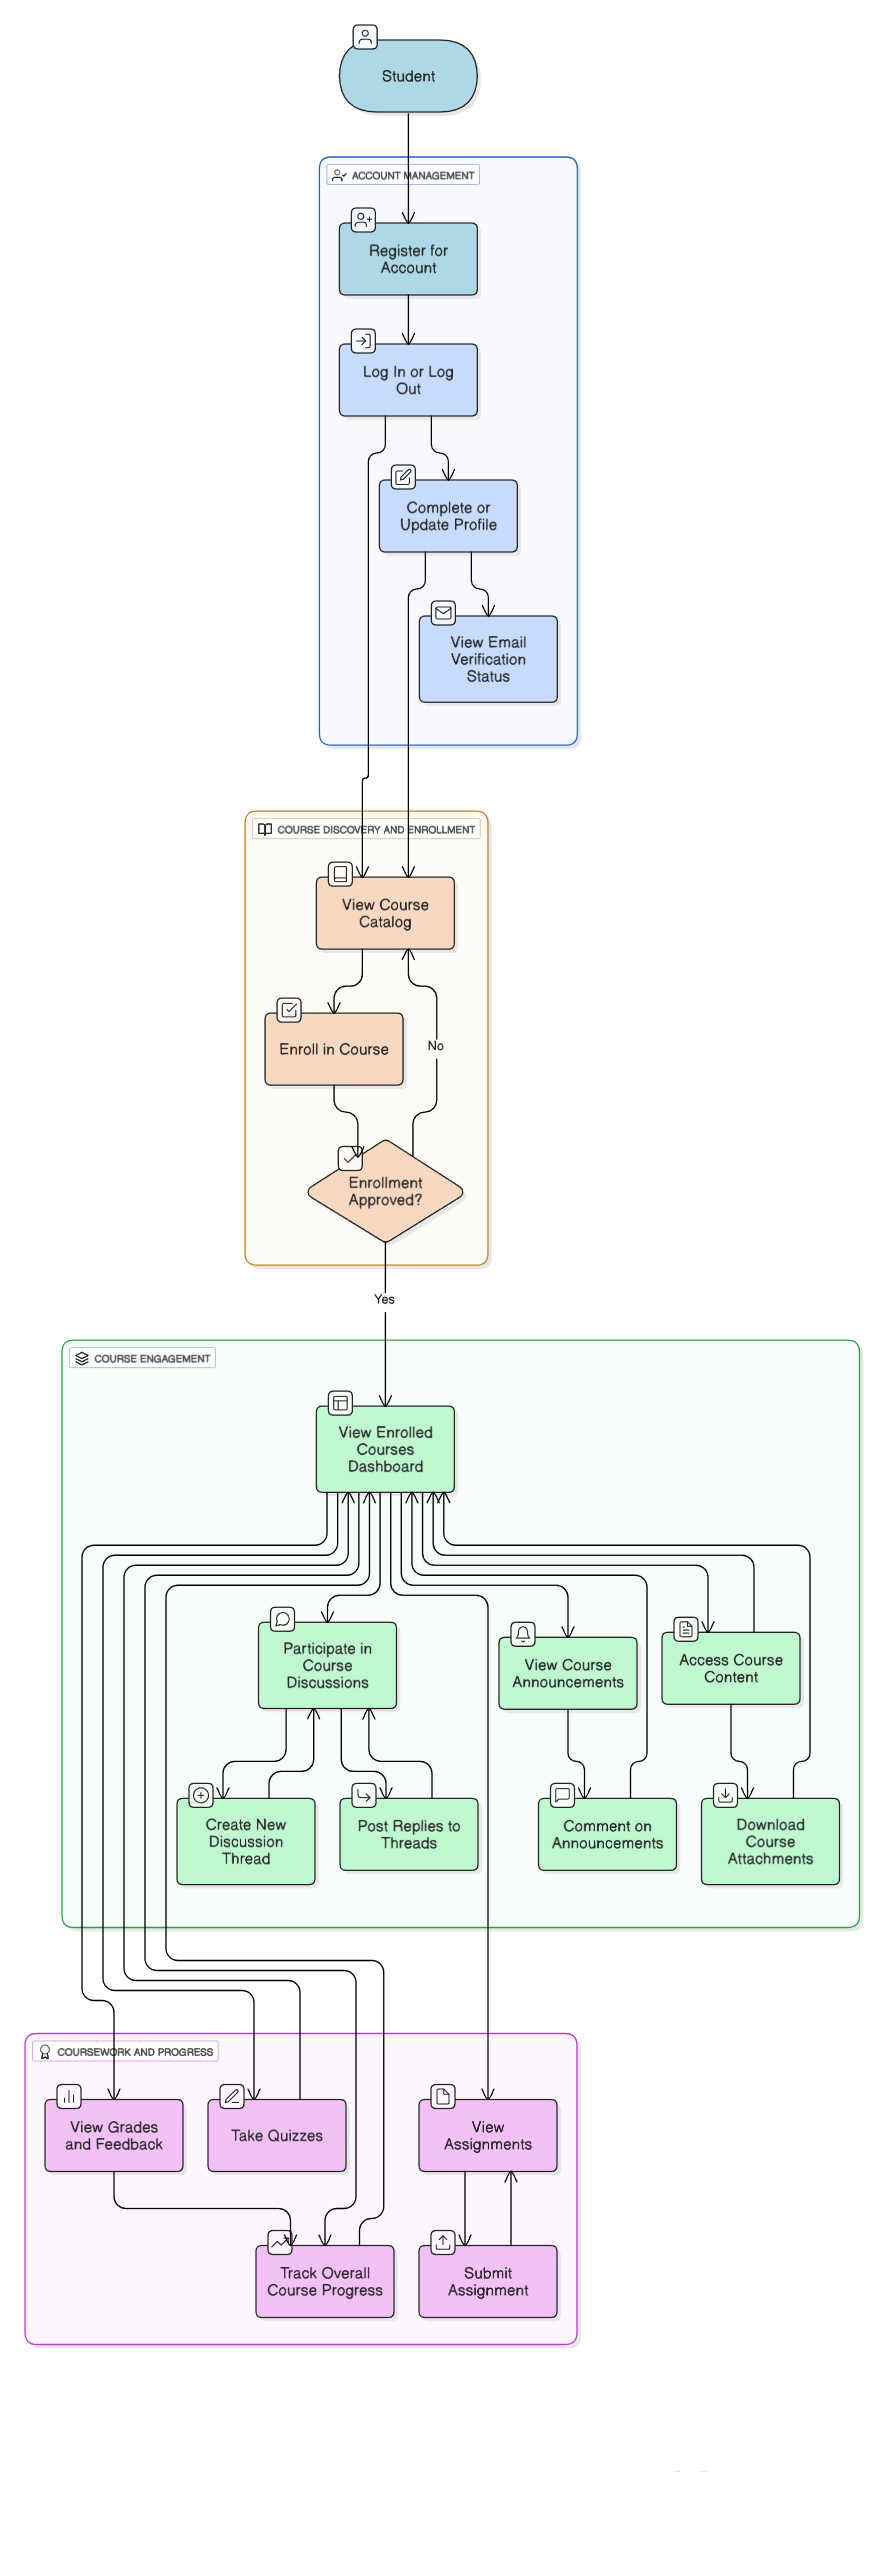
\includegraphics[width=0.8\textwidth,height=0.85\textheight,keepaspectratio]{student-usecase-diagram.png}
        \captionof{figure}{Student Use Case Diagram - showing interactions between students and the learning platform}
        \label{fig:student-usecase}
    \end{center}
    \clearpage

    \item \textbf{Instructor Use Case Diagram}
    
    \begin{figure}[!htbp]
        \centering
        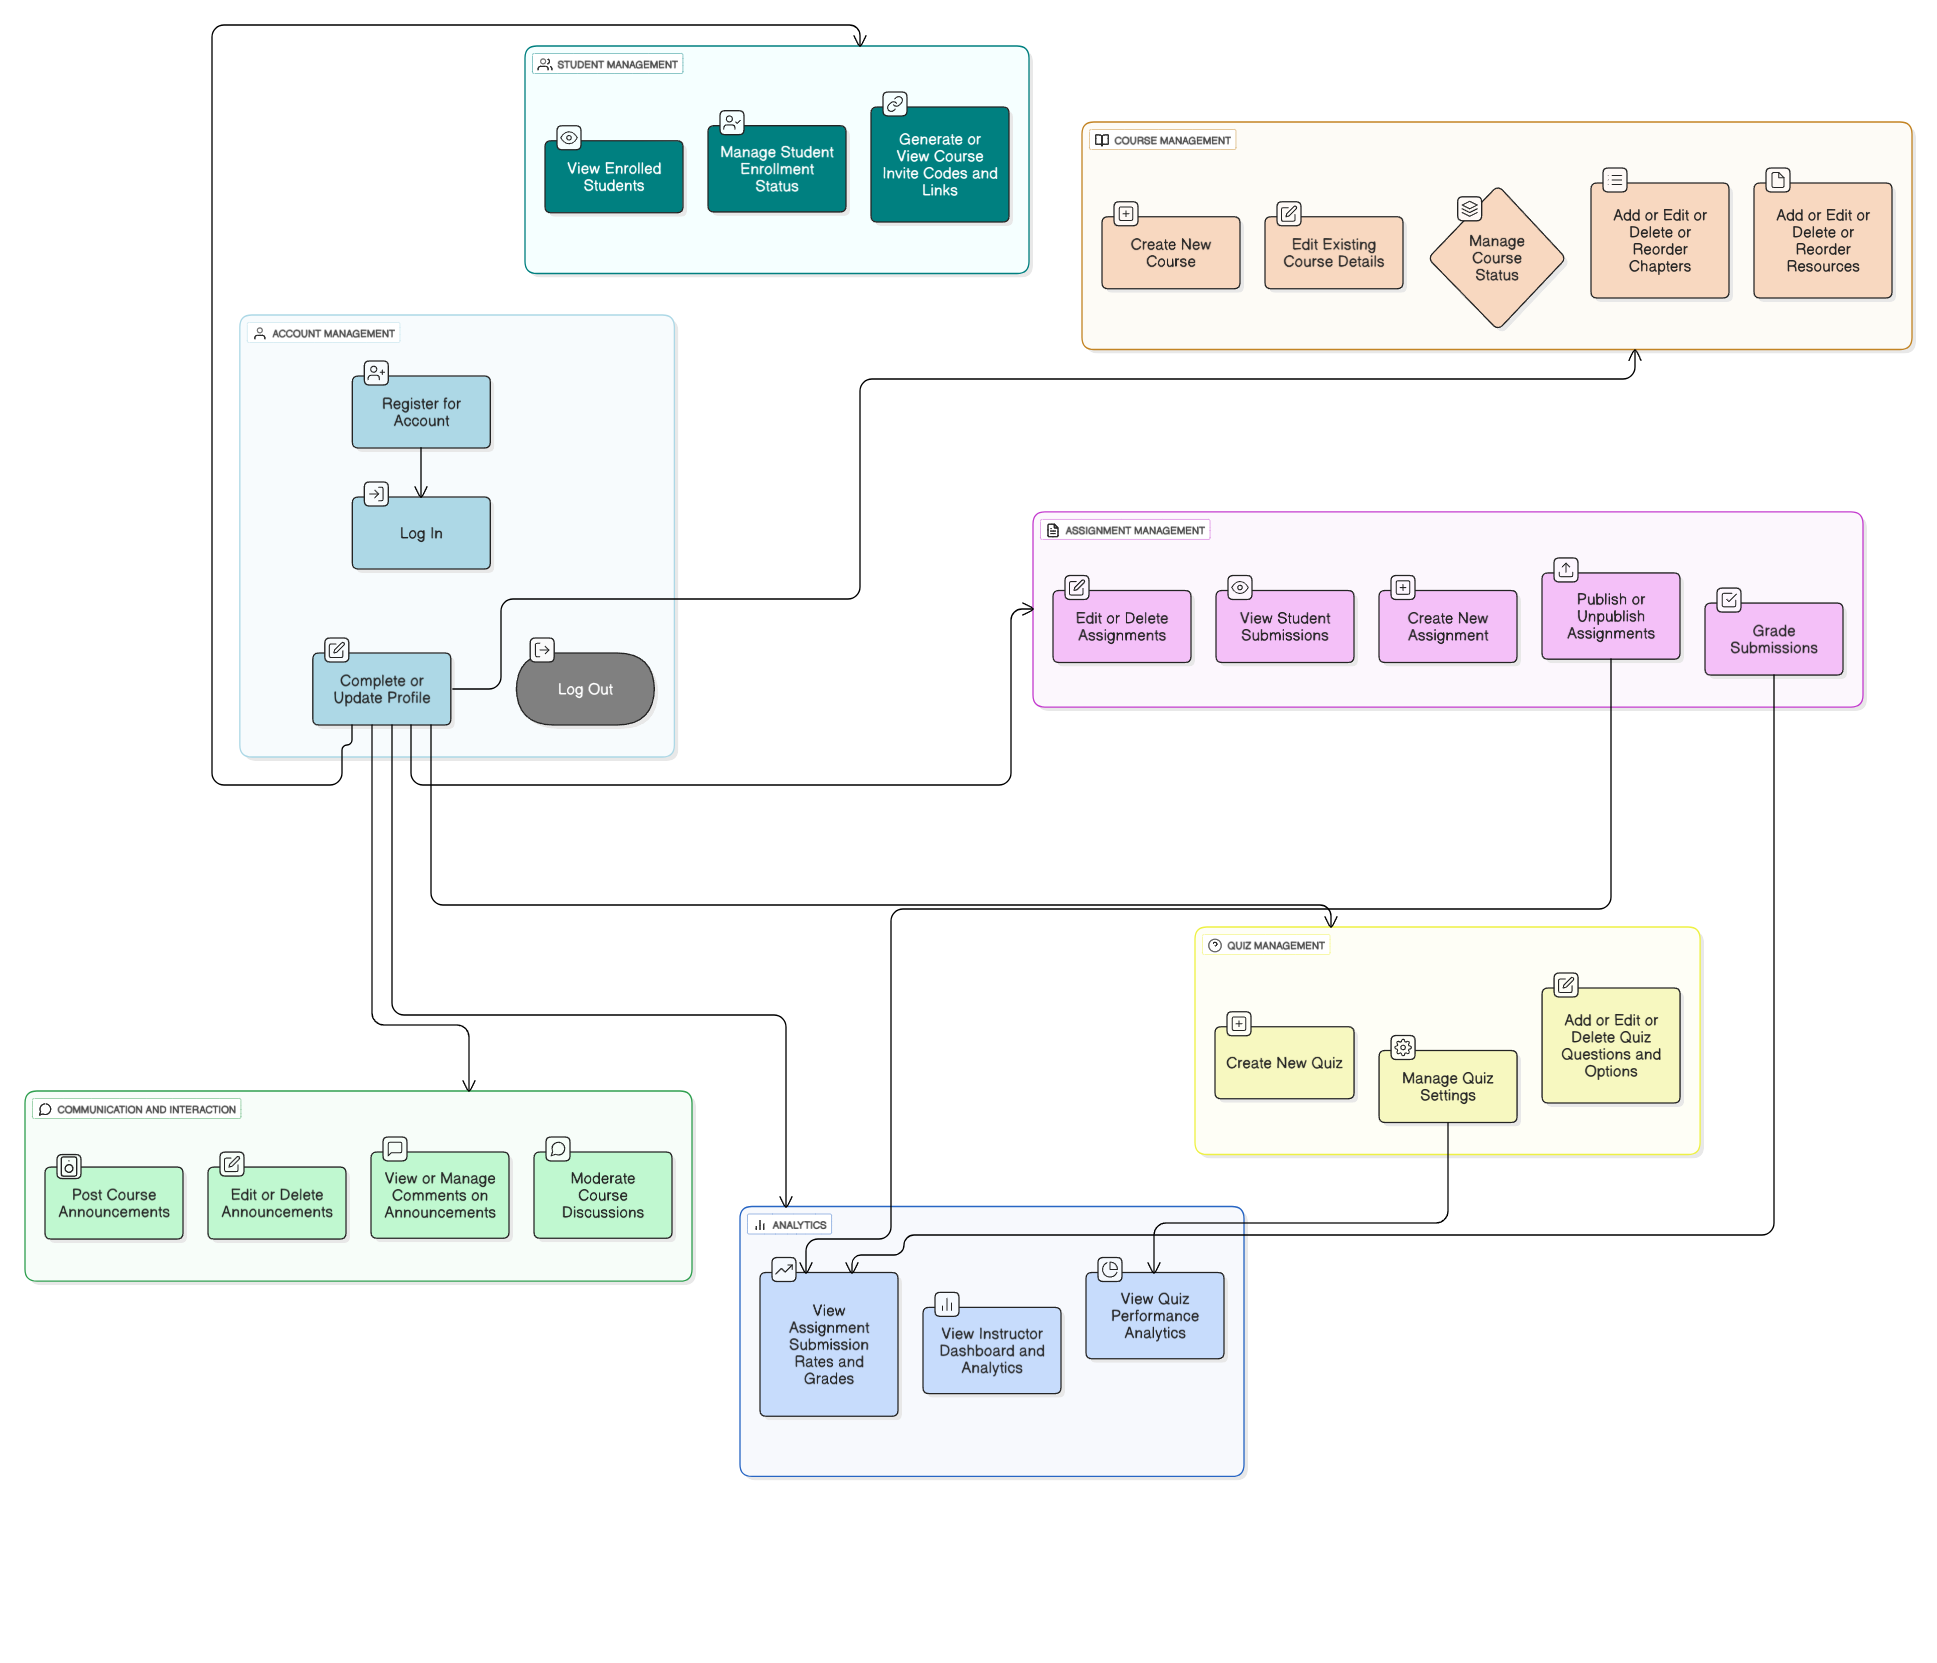
\includegraphics[width=0.9\textwidth]{instructor-usecase-diagram.png}
        \caption{Instructor Use Case Diagram - illustrating instructor functionalities and system interactions}
        \label{fig:instructor-usecase}
    \end{figure}
    \FloatBarrier

    \item \textbf{Administrator Use Case Diagram}
    
    \begin{figure}[!htbp]
        \centering
        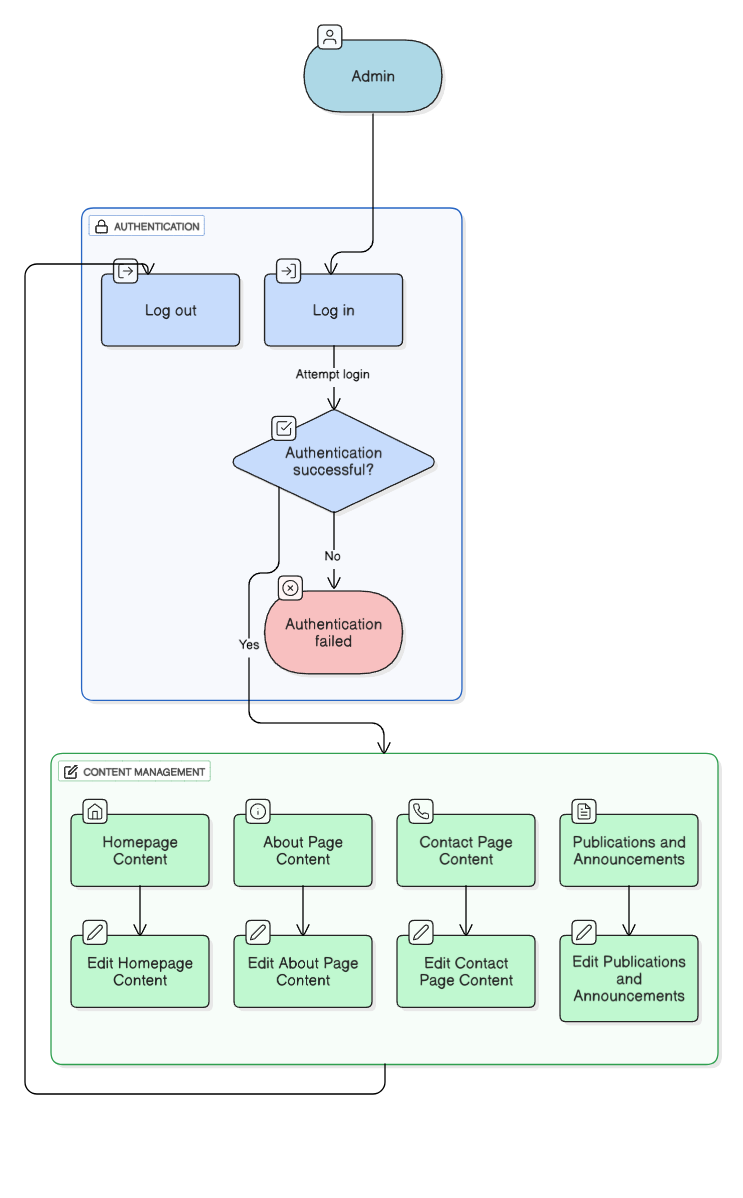
\includegraphics[width=0.9\textwidth]{administrator-usecase-diagram.png}
        \caption{Administrator Use Case Diagram - depicting administrative operations and system management tasks}
        \label{fig:administrator-usecase}
    \end{figure}
    \FloatBarrier
\end{itemize}

\subsection{Sequence Diagrams}

These diagrams trace the flow of information through the system during critical operations, revealing the intricate coordination between frontend, backend, and data storage components:

\begin{itemize}
    \item \textbf{Student Submits Assignment:}
    \begin{center}       
        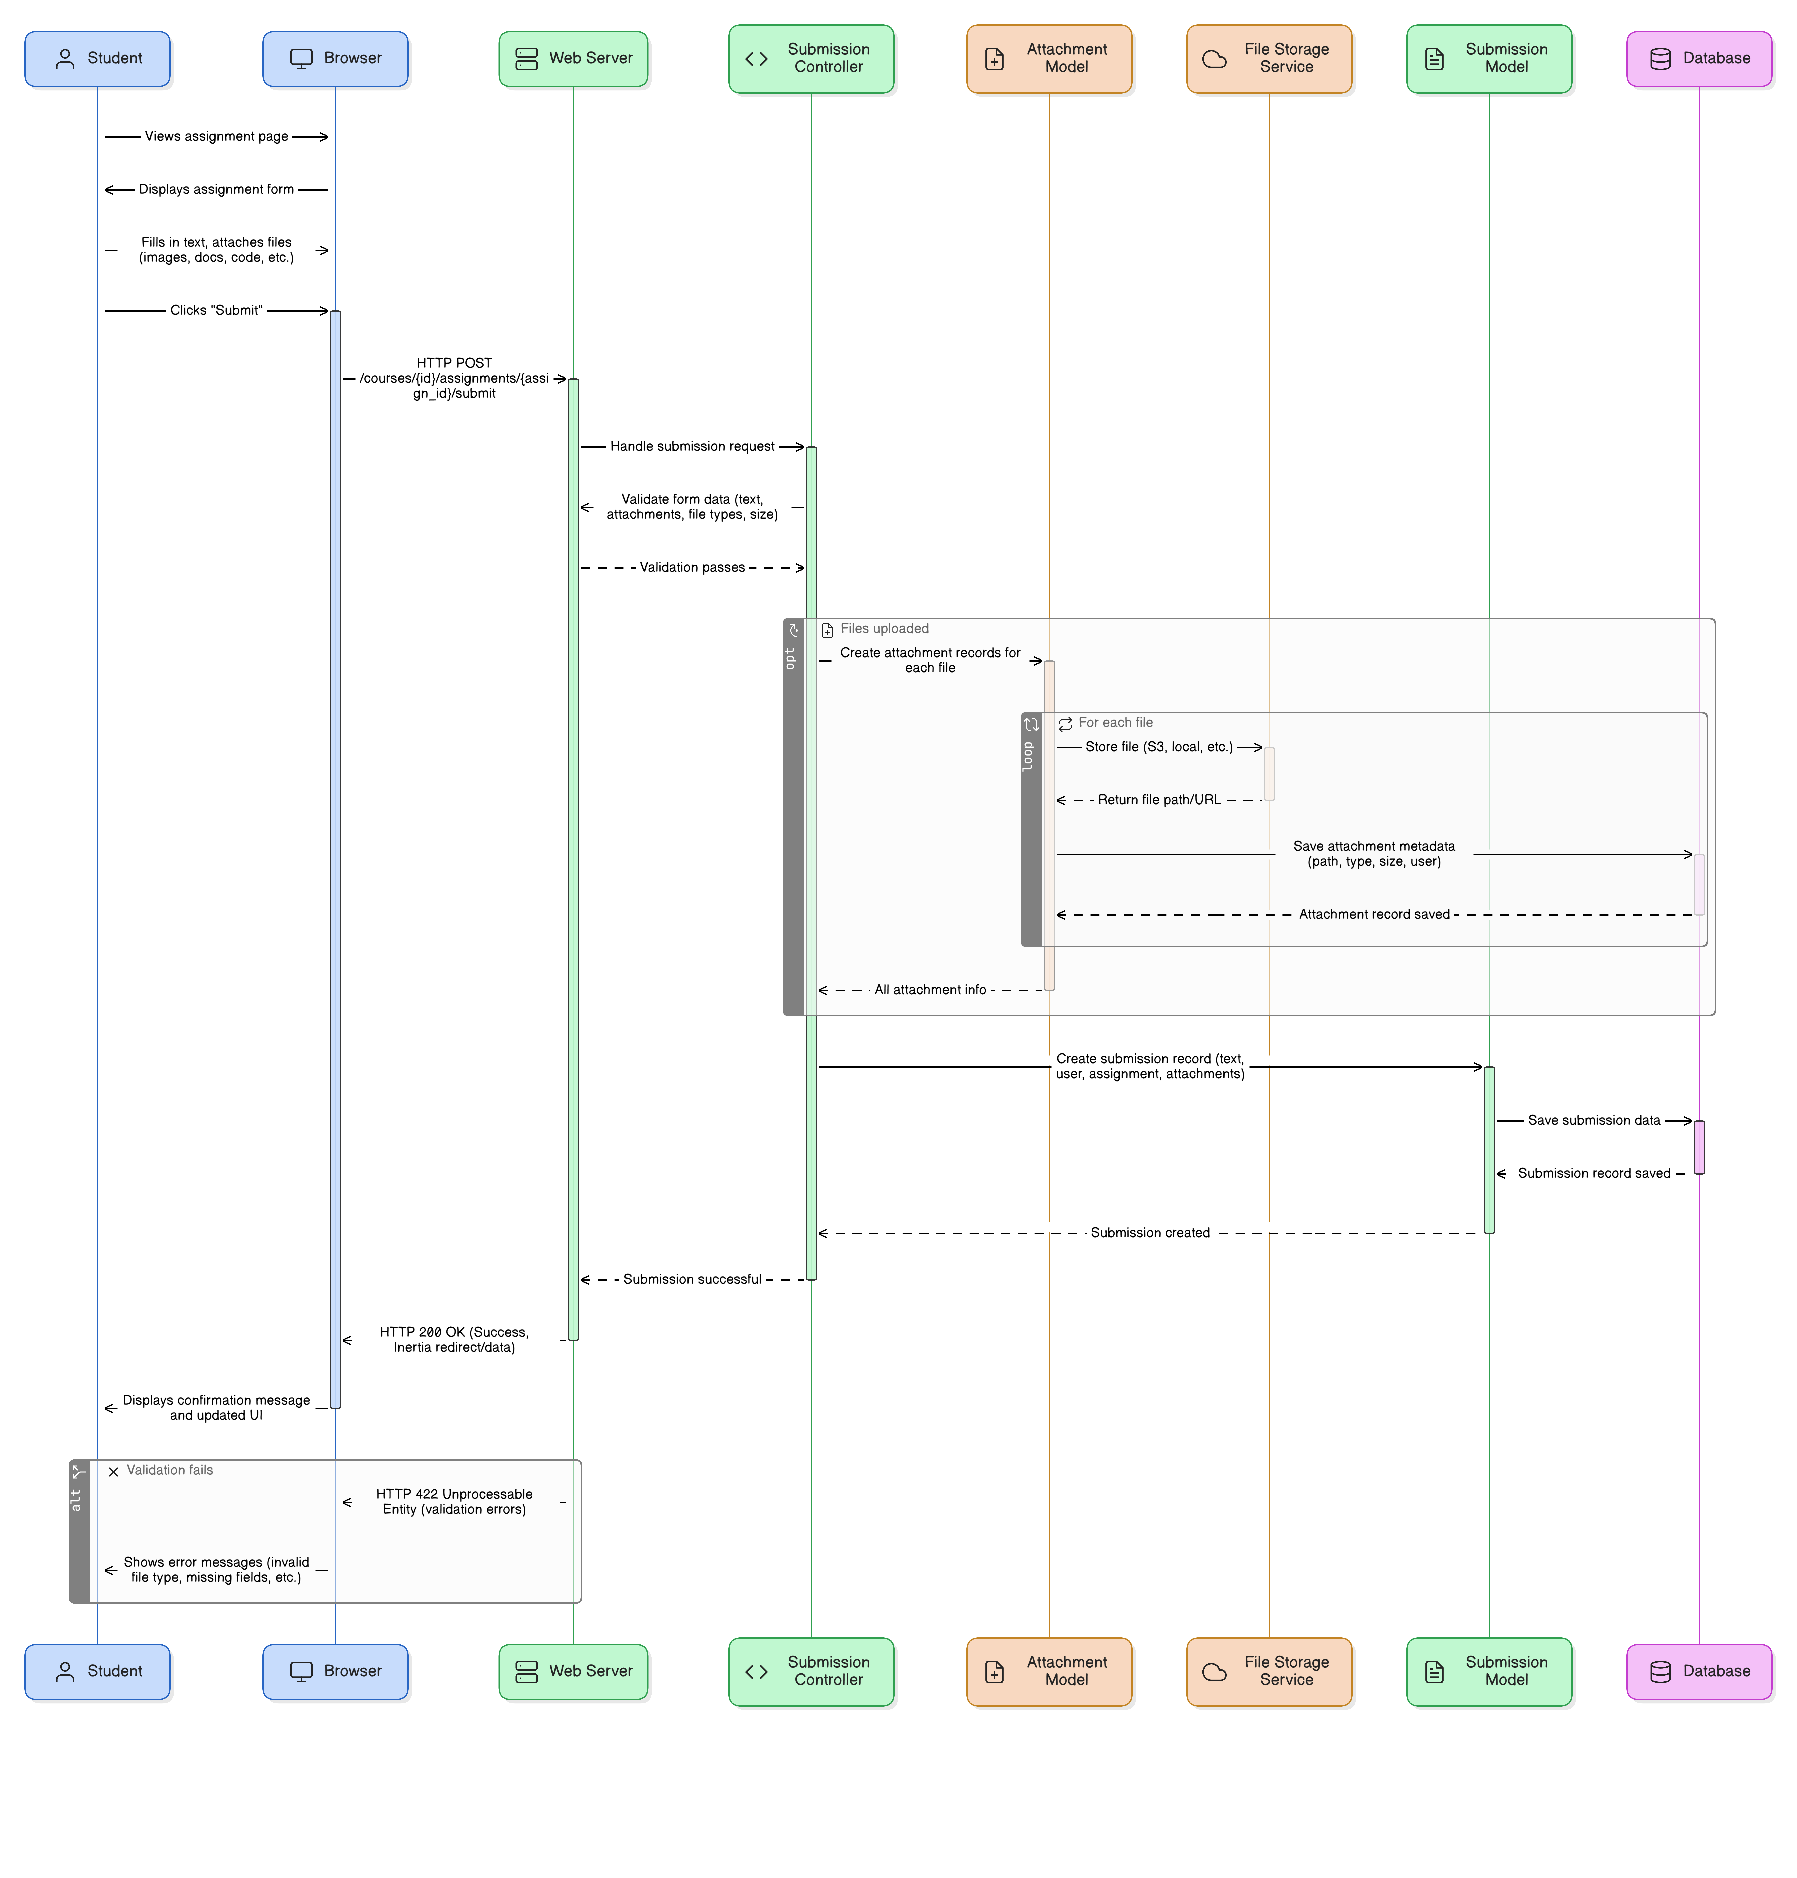
\includegraphics[width=0.8\textwidth,height=0.85\textheight,keepaspectratio]{student-submits-assignment.png}
        \captionof{figure}{Student assignment submission sequence diagram}
        \label{fig:student-submits-assignment}
        \end{center}
    \clearpage
    \item \textbf{Instructor Grades Submission:}
    \begin{center}       
        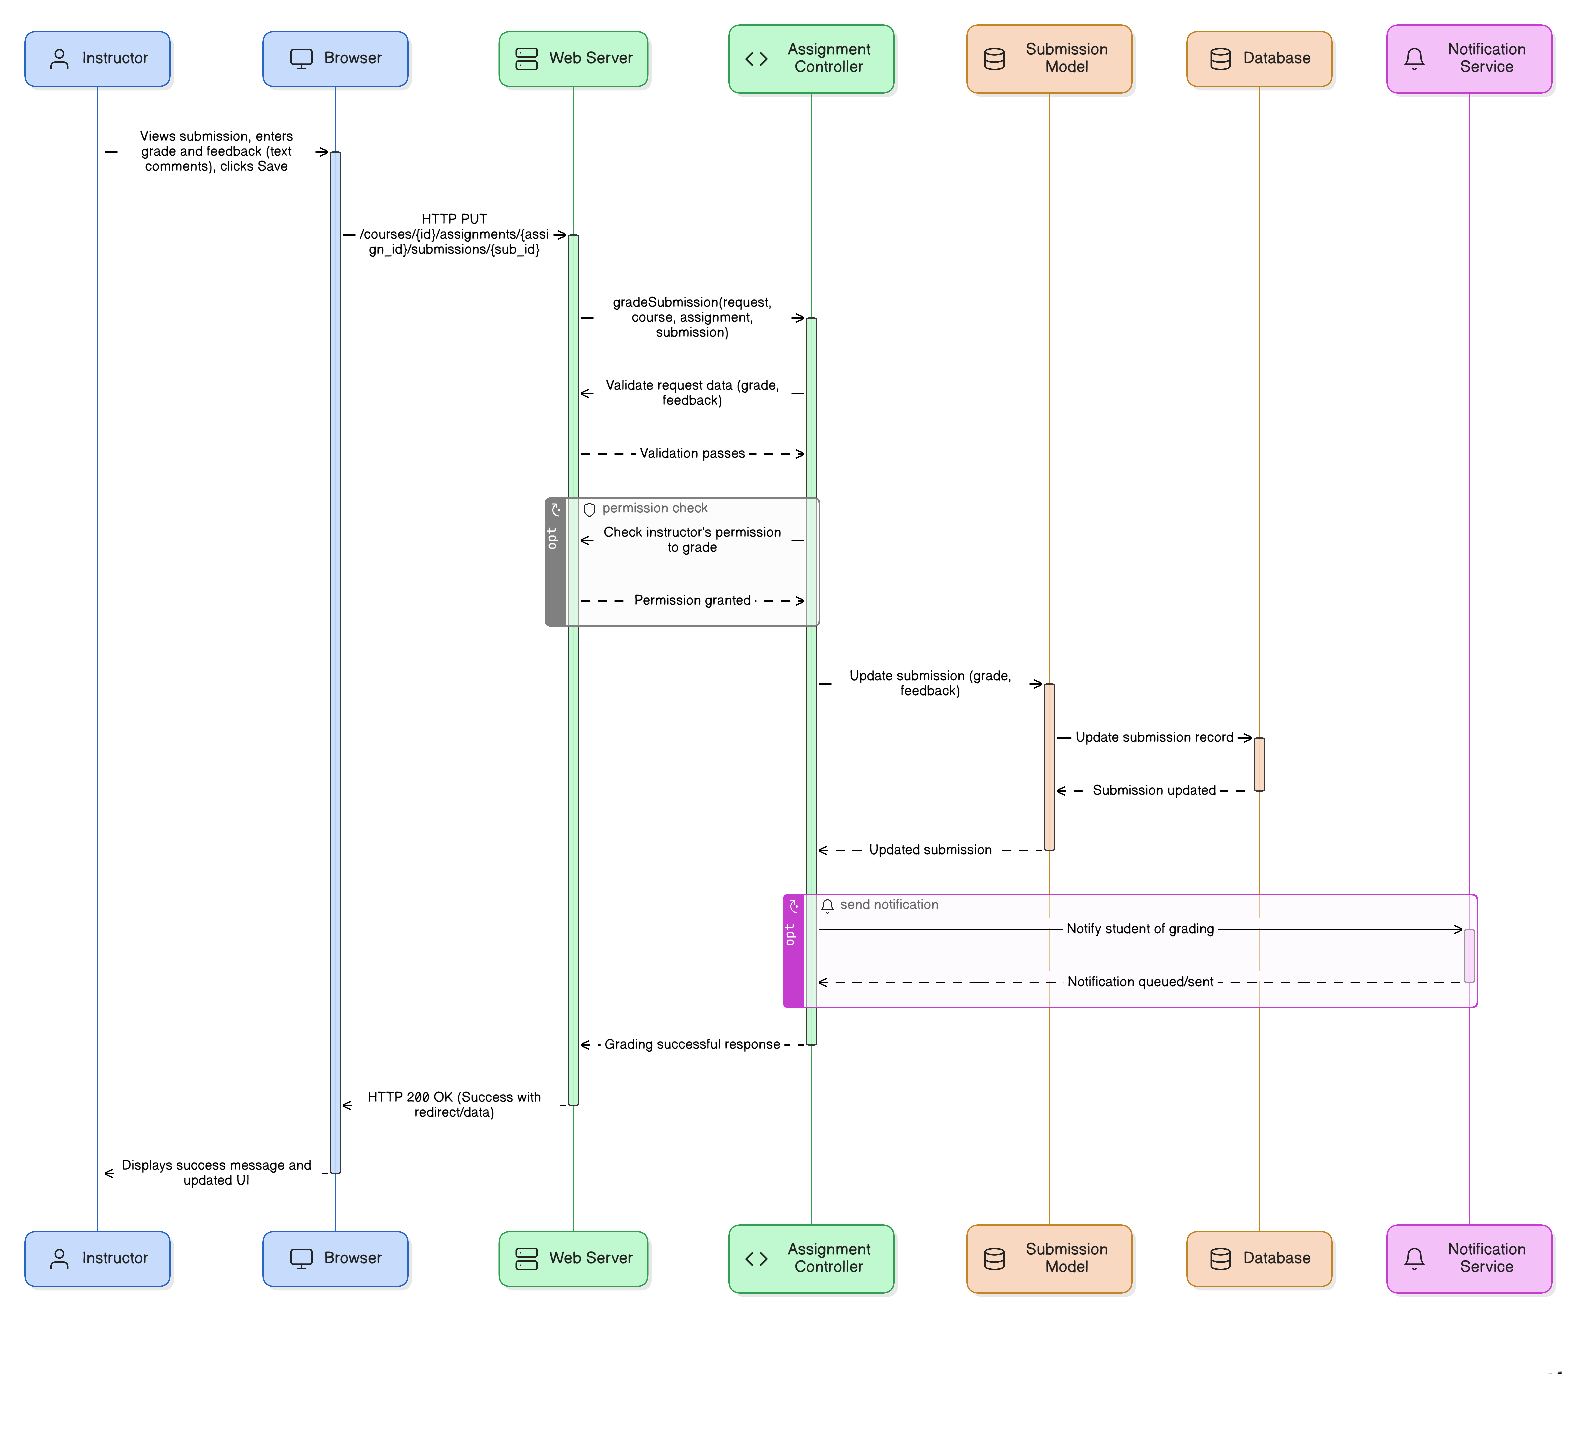
\includegraphics[width=0.8\textwidth,height=0.85\textheight,keepaspectratio]{instructor-grades-submission.png}
        \captionof{figure}{Instructor grading a submission sequence diagram}
        \label{fig:instructor-grades-submission}
        \end{center}
    \clearpage
    \item \textbf{User (Student/Instructor) Authenticates (Login):}
    \begin{center}       
        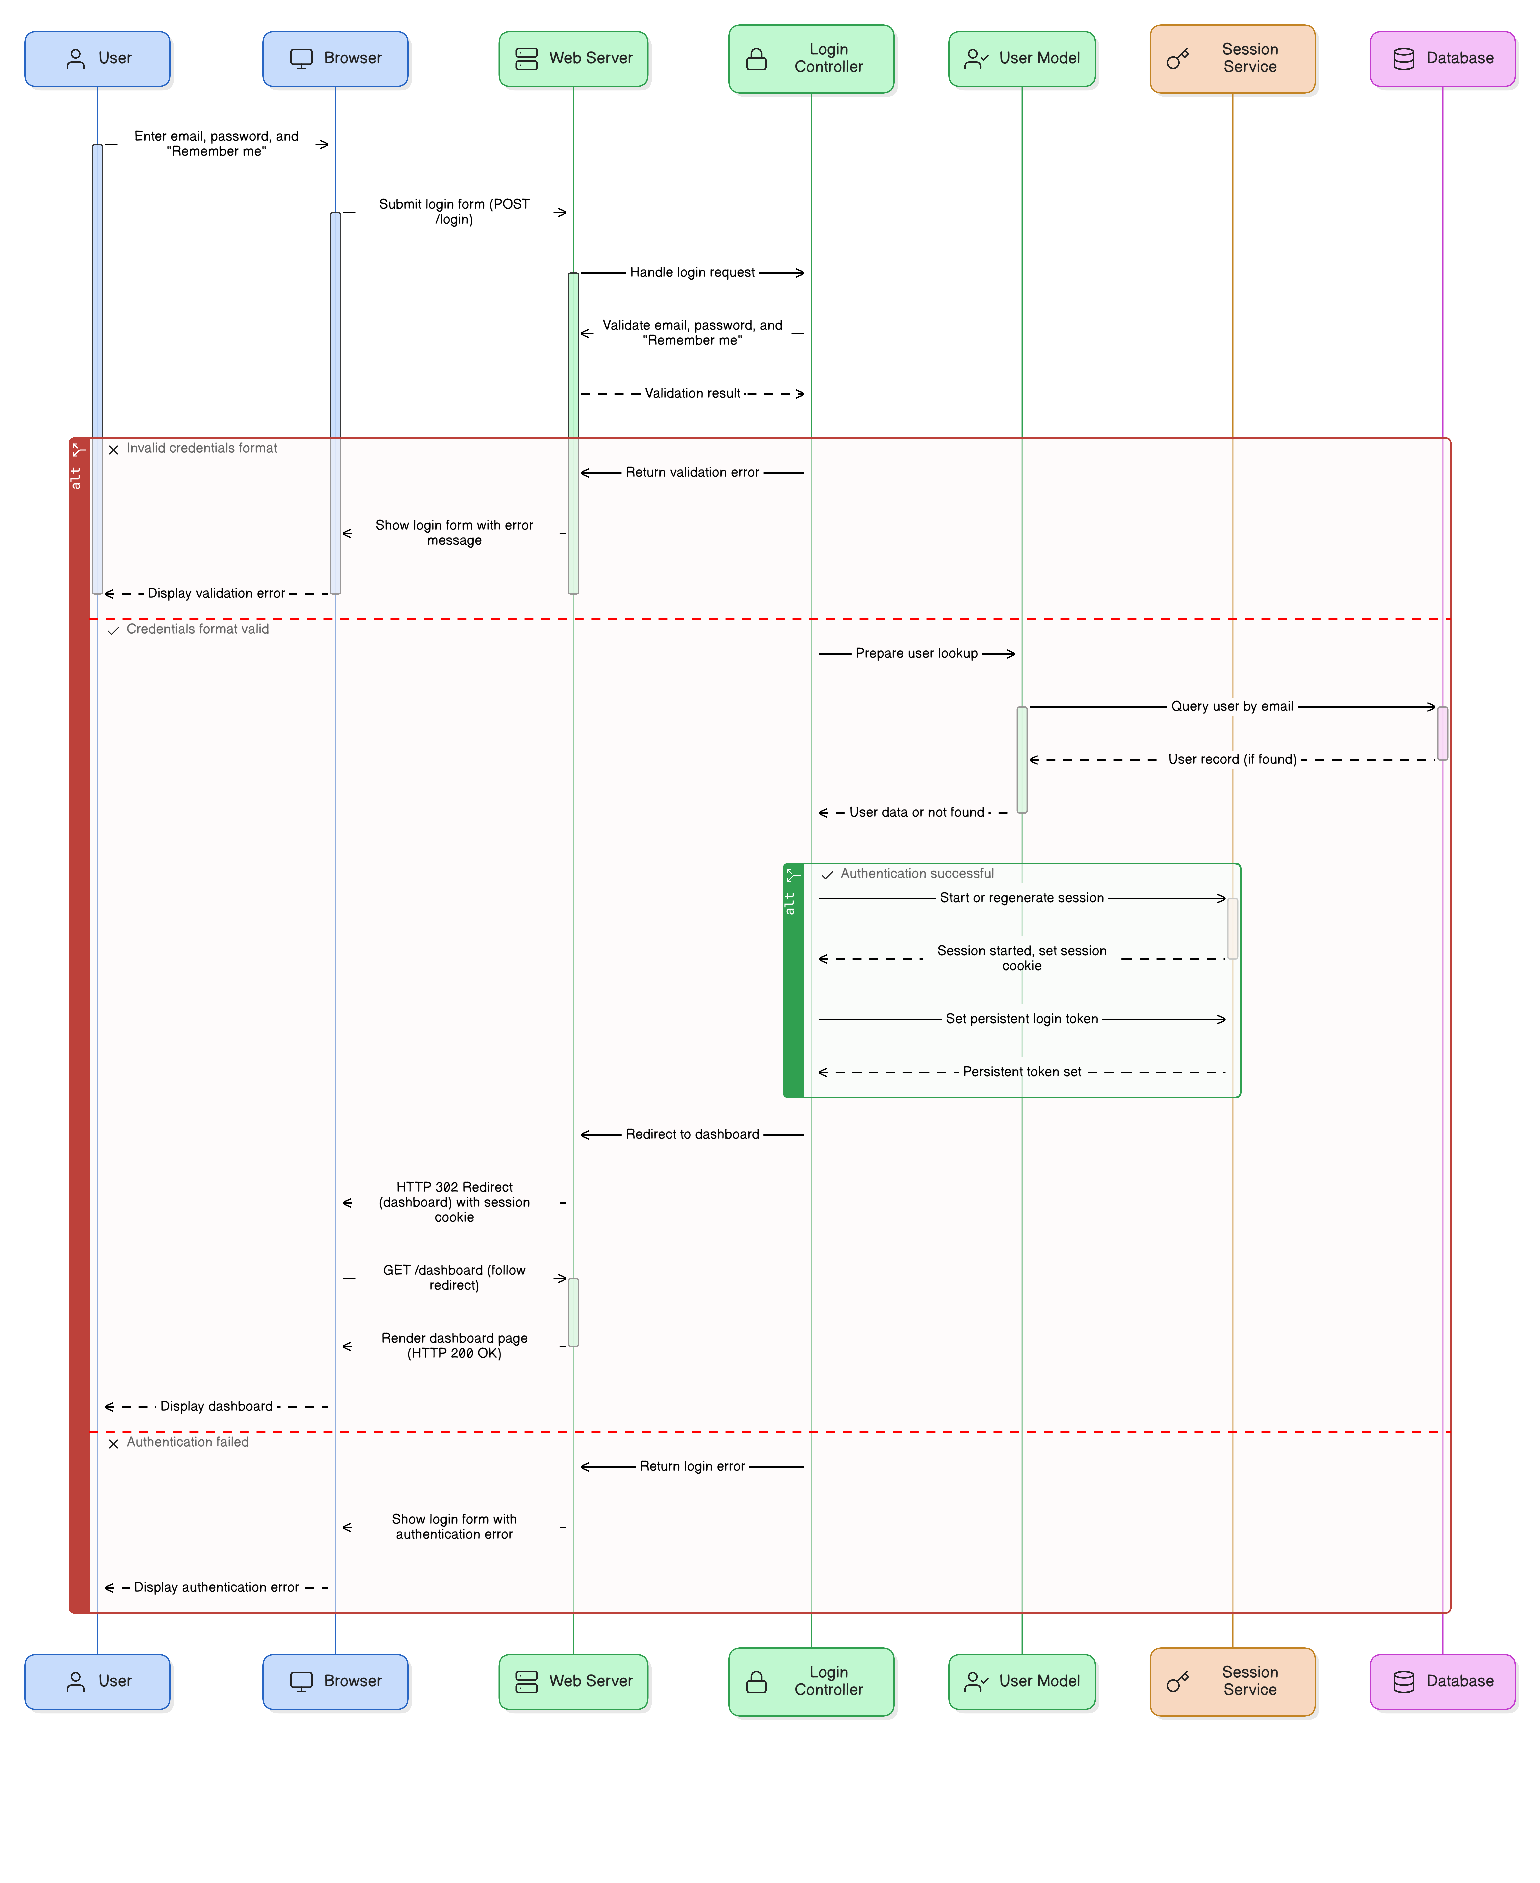
\includegraphics[width=0.8\textwidth,height=0.85\textheight,keepaspectratio]{user-authentication.png}
        \captionof{figure}{User authentication sequence diagram}
        \label{fig:user-authentication}
        \end{center}
    \clearpage
\end{itemize}

\subsection{System Architecture Overview}

This diagram presents the platform's technical architecture, illustrating how different software layers interact to deliver the complete user experience:

\begin{itemize}
    \item \textbf{Components:}
        \begin{center}       
        \includegraphics[width=0.8\textwidth,height=0.85\textheight,keepaspectratio]{system-architecture-overview.png}
        \captionof{figure}{System Architecture flowchart}
        \label{fig:system-architecture-overview}
        \end{center}
    \begin{itemize}
        \item \textbf{Client Tier:}
        \begin{itemize}
            \item \textbf{Web Browser:} Renders the UI (React components via Inertia.js), handles user input, executes client-side JavaScript.
        \end{itemize}
        \item \textbf{Application Tier:}
        \begin{itemize}
            \item \textbf{Web Server (e.g., Nginx, Apache):} Receives HTTP requests, serves static assets, acts as a reverse proxy for the application.
            \item \textbf{Laravel Application (PHP-FPM):}
            \begin{itemize}
                \item \textbf{Routing Engine:} Maps URLs to controller actions.
                \item \textbf{Controllers:} Handle HTTP requests, interact with models and services, prepare data for views/Inertia responses.
                \item \textbf{Models (Eloquent ORM):} Represent database tables, manage data persistence and relationships.
                \item \textbf{Middleware:} Handles cross-cutting concerns (authentication, CSRF, Inertia requests).
                \item \textbf{Inertia.js Adapter:} Bridges Laravel backend with React frontend.
                \item \textbf{Services:} Encapsulate specific business logic (e.g., QuizService, NotificationService - if explicitly created).
            \end{itemize}
        \end{itemize}
        \item \textbf{Data Tier:}
        \begin{itemize}
            \item \textbf{Database Server (e.g., MySQL, PostgreSQL, SQLite):} Stores all persistent application data (users, courses, submissions, etc.).
            \item \textbf{Cache Server (e.g., Redis):} Stores session data, cached queries, etc.
        \end{itemize}
        \item \textbf{External Services / Storage:}
        \begin{itemize}
            \item \textbf{File Storage (AWS S3):} Stores user-uploaded files (avatars, course materials, assignment attachments).
            \item \textbf{Email Service:} For sending transactional emails (verification, notifications).
        \end{itemize}
    \end{itemize}
    \item \textbf{Key Interactions:}
    \begin{itemize}
        \item Browser \texttt{<->} Web Server (HTTP/HTTPS)
        \item Web Server \texttt{<->} Laravel Application (FastCGI/PHP-FPM)
        \item Laravel Application \texttt{<->} Database Server (SQL)
        \item Laravel Application \texttt{<->} Cache Server
        \item Laravel Application \texttt{<->} File Storage
    \end{itemize}
\end{itemize}

\section{Technologies and Tools Used}

The platform's technical foundation reflects careful consideration of performance, maintainability, and developer experience. Each technology choice contributes to a cohesive development environment that supports rapid iteration while ensuring production reliability:

\subsection*{Backend}

\begin{itemize}
    \item \textbf{Programming Language:} PHP (Version 8.3+)
    \item \textbf{Framework:} Laravel (Version 12)
    \item \textbf{Key PHP Libraries \& Packages:}
    \begin{itemize}
        \item \texttt{inertiajs/inertia-laravel}: Server-side adapter for Inertia.js, facilitating integration with the React frontend.
        \item \texttt{prism-php/prism}: Laravel package for integrating Large Language Models (LLMs).
        \item \texttt{tightenco/ziggy}: Enables the use of Laravel named routes within JavaScript.
        \item \texttt{league/flysystem-aws-s3-v3}: Provides an abstraction for file storage, configured for AWS S3. (Also supports local and other drivers).
        \item \texttt{predis/predis}: A flexible and feature-complete Redis client for PHP.
    \end{itemize}
\end{itemize}

\subsection*{Frontend}

\begin{itemize}
    \item \textbf{Programming Languages:} TypeScript, JavaScript (ES6+)
    \item \textbf{Framework/Library:} React (Version 19)
    \item \textbf{SPA Integration:} Inertia.js (using \texttt{@inertiajs/react} adapter) for building a modern, single-page application experience with server-driven routing.
    \item \textbf{Key JavaScript Libraries \& Packages:}
    \begin{itemize}
        \item \textbf{UI \& Components:}
        \begin{itemize}
            \item \texttt{@radix-ui/*}: A comprehensive suite of unstyled, accessible UI primitives (e.g., Dialog, Dropdown, Select, Tooltip) used as the foundation for custom components (likely following a Shadcn UI-like pattern).
            \item \texttt{lucide-react}: For a wide range of SVG icons.
            \item \texttt{@headlessui/react}: Unstyled, fully accessible UI components.
            \item \texttt{cmdk}: Command menu component for quick navigation and actions.
            \item \texttt{embla-carousel-react}: A bare-bones carousel library.
            \item \texttt{sonner}: For displaying toast notifications.
            \item \texttt{recharts}: A composable charting library.
            \item \texttt{react-day-picker}: Date picker component.
            \item \texttt{vaul}: Drawer component.
        \end{itemize}
        \item \textbf{Text Editing:}
        \begin{itemize}
            \item \texttt{@tiptap/react} \& extensions: A headless, framework-agnostic rich text editor.
        \end{itemize}
        \item \textbf{Drag \& Drop:}
        \begin{itemize}
            \item \texttt{@dnd-kit/core} \& \texttt{@dnd-kit/sortable}: For implementing drag and drop interfaces.
        \end{itemize}
        \item \textbf{Forms \& Validation:}
        \begin{itemize}
            \item \texttt{zod} \& \texttt{zod-form-data}: For robust schema definition and validation.
            \item \texttt{react-dropzone}: For handling file uploads via drag and drop.
            \item \texttt{input-otp}: One-time password input component.
        \end{itemize}
        \item \textbf{Tables:}
        \begin{itemize}
            \item \texttt{@tanstack/react-table}: Headless UI for building powerful tables and datagrids.
        \end{itemize}
        \item \textbf{Animation:}
        \begin{itemize}
            \item \texttt{framer-motion}: A production-ready motion library for React.
        \end{itemize}
        \item \textbf{Utilities:}
        \begin{itemize}
            \item \texttt{date-fns}: Modern JavaScript date utility library.
            \item \texttt{next-themes}: For theme management (e.g., light/dark mode).
        \end{itemize}
    \end{itemize}
\end{itemize}

\subsection*{Database}

\begin{itemize}
    \item \textbf{Development Default:} SQLite
    \item \textbf{Production Options:} MySQL, MariaDB, PostgreSQL, SQL Server (as per Laravel's standard support and \texttt{config/database.php}).
    \item \textbf{Caching / Key-Value Store:} Redis (client \texttt{predis/predis} configured).
\end{itemize}

\subsection*{Styling}

\begin{itemize}
    \item \textbf{CSS Framework:} Tailwind CSS (Version 4)
    \item \textbf{Utility Libraries:}
    \begin{itemize}
        \item \texttt{class-variance-authority} (CVA): For creating type-safe, reusable UI components with variants.
        \item \texttt{clsx}: A tiny utility for constructing \texttt{className} strings conditionally.
        \item \texttt{tailwind-merge}: Utility to merge Tailwind CSS classes without style conflicts.
        \item \texttt{tailwindcss-animate}: Plugin for Tailwind CSS that adds enter/exit animations.
        \item \texttt{@tailwindcss/typography}: Tailwind CSS plugin for styling prose/HTML content.
    \end{itemize}
\end{itemize}

\subsection*{Build \& Development Tools}

\begin{itemize}
    \item \textbf{JavaScript Bundler \& Dev Server:} Vite
    \item \textbf{PHP Dependency Manager:} Composer
    \item \textbf{JavaScript Package Manager:} npm (inferred from \texttt{package-lock.json}, though \texttt{bun.lock} also exists, indicating Bun might be used by some developers or in CI).
    \item \textbf{Version Control:} Git
    \item \textbf{Local Development Environment:} Laravel Sail (Docker-based, provides a standardized local development experience).
    \item \textbf{Debugging (Backend):} \texttt{barryvdh/laravel-debugbar} for in-browser debugging information.
    \item \textbf{Linters \& Formatters:}
    \begin{itemize}
        \item ESLint (JavaScript/TypeScript linter)
        \item Prettier (Code formatter)
        \item Laravel Pint (PHP code style fixer)
    \end{itemize}
\end{itemize}

\subsection*{Testing}

\begin{itemize}
    \item \textbf{PHP Unit \& Feature Testing:} Pest (built on top of PHPUnit).
    \item \textit{(Frontend testing tools like Jest or React Testing Library were not explicitly listed in the primary \texttt{package.json} devDependencies. Testing strategy for the frontend is not detailed from the provided file analysis.)}
\end{itemize}

\subsection*{Server Environment (Typical Deployment)}

\begin{itemize}
    \item \textbf{Web Server:} Nginx or Apache
    \item \textbf{PHP Runtime:} PHP-FPM (FastCGI Process Manager)
    \item \textbf{Database Server:} (MySQL Server)
    \item \textbf{Node.js:} Required for the frontend build process.
\end{itemize}

\section{User Interface Design}

The following screenshots provide a comprehensive view of the platform's user interface design and functionality. Each screen demonstrates the practical implementation of the features described in previous sections, showing how users interact with the system across different roles and contexts:

\subsection{Public Pages}

These pages are accessible to all visitors and are primarily rendered using Laravel Blade views, with dynamic content fetched from the database. The course listing page might be enhanced with React/Inertia for dynamic filtering and display.

\begin{itemize}
    \item \textbf{Homepage (\texttt{home.blade.php}):}
    \begin{itemize}
        \item \textbf{Layout:} A clean and modern design featuring a prominent header and a comprehensive footer.
        \begin{itemize}
            \item \textit{Header:} Contains the ENSIASD logo, navigation links (Home, Courses, Publications, About, Contact), and buttons for "Login" and "Register".
            \item \textit{Footer:} Includes copyright information, links to social media, and possibly quick links to important sections.
        \end{itemize}
        \item \textbf{Content Sections:}
        \begin{itemize}
            \item \textit{Hero Section:} A full-width banner with a captivating background image (dynamically set from \texttt{HomeContent}). Overlayed text includes a welcoming title (e.g., "Empowering Education Through Technology") and a brief description of the platform, both dynamic. Two prominent call-to-action buttons like "Explore Courses" (linking to the course listing) and "Learn More" (linking to the About page).
            \item \textit{Popular Courses:} A section titled "Browse Our Popular Courses". Displays 3-4 course cards in a grid. Each card features a course image, category, title, a short description, the instructor's name and avatar, and a "View Course" link.
            \item \textit{Platform Features ("Why Choose Us"):} A section highlighting key benefits, presented as a grid of feature cards. Each card has an icon (e.g., \texttt{fas fa-laptop-code} for Interactive Learning), a feature title, and a short explanatory text. Examples: "Interactive Learning," "Expert Instructors," "Flexible Schedule," "Certification."
            \item \textit{Call to Action (CTA):} A visually distinct section encouraging user registration, with a title like "Ready to Start Learning?" and buttons for "Register Now" and "Contact Us."
        \end{itemize}
    \end{itemize}
    \item \textbf{Course Listing Page (\texttt{courses.blade.php}, potentially with React/Inertia):}
    \begin{itemize}
        \item \textbf{Layout:} Standard header and footer. The main content area is dedicated to displaying courses.
        \item \textbf{Content:}
        \begin{itemize}
            \item \textit{Search and Filters:} A search bar at the top allows users to search for courses by title, description, or category. Filter dropdowns or sidebar options might be available for filtering by "Category."
            \item \textit{Course Grid/List:} Courses are displayed in a responsive grid or list format. Each course card prominently shows its image, title, category, the instructor's name, and possibly the number of enrolled students or a rating. A button or link on each card leads to the detailed course view (if public) or prompts login.
            \item \textit{Pagination:} If there are many courses, pagination controls are visible at the bottom.
            \item \textit{No Results Message:} A user-friendly message and illustration (e.g., \texttt{nothing-found.svg}) appear if no courses match the search/filter criteria.
        \end{itemize}
    \end{itemize}
    \item \textbf{About Page (\texttt{about.blade.php}):}
    \begin{itemize}
        \item \textbf{Layout:} Standard header and footer.
        \item \textbf{Content (Dynamically loaded from \texttt{AboutContent} model):}
        \begin{itemize}
            \item \textit{Hero Section:} Similar to the homepage hero, with a title like "About Our Platform" and relevant imagery.
            \item \textit{Mission/Vision:} Dedicated sections with text describing the platform's mission and vision, possibly accompanied by images.
            \item \textit{Platform Features:} Detailed descriptions of platform features (e.g., "Virtual Classes," "Centralized Resources," "Assignment Management").
            \item \textit{Statistics:} A visually engaging display of platform statistics (e.g., "Active Courses," "Teachers," "Students," "Satisfaction Rate").
            \item \textit{Benefits:} Sections detailing benefits for teachers and students, presented as bullet points or featurettes.
        \end{itemize}
    \end{itemize}
    \item \textbf{Contact Page (\texttt{contact.blade.php}):}
    \begin{itemize}
        \item \textbf{Layout:} Standard header and footer.
        \item \textbf{Content (Dynamically loaded from \texttt{ContactContent} model):}
        \begin{itemize}
            \item \textit{Contact Information:} Clearly displayed school name, address, phone number, and email address.
            \item \textit{Office Hours:} Information on when users can expect support or contact the institution.
            \item \textit{Contact Form (Implied or possible):} A form for users to send inquiries directly.
            \item \textit{Embedded Map:} An interactive map (e.g., Google Maps iframe) showing the institution's location.
            \item \textit{Contact Image:} A relevant image for the contact page.
        \end{itemize}
    \end{itemize}
    \item \textbf{Publications Page (\texttt{publications.blade.php}):}
    \begin{itemize}
        \item \textbf{Layout:} Standard header and footer.
        \item \textbf{Content:} A list or grid of articles, news, or general announcements (from the \texttt{Announcement} model, possibly filtered for site-wide items or a specific "Publications" category).
        \begin{itemize}
            \item Each item displays a title, a snippet of the content or a summary, the publication date, author (if applicable), and potentially an associated course.
            \item Clicking an item would lead to a detailed view of that publication/announcement.
        \end{itemize}
    \end{itemize}
\end{itemize}

\subsection{Authenticated User Dashboard \& Internal Pages (React/Inertia)}

These pages are part of the SPA experience after a user logs in, built with React and Inertia.js. They feature a consistent application shell.

\begin{itemize}
    \item \textbf{Main Dashboard Layout (\texttt{AppLayout.tsx}):}
    \begin{itemize}
        \item \textbf{Application Shell:}
        \begin{itemize}
            \item \textit{Sidebar (\texttt{AppSidebar.tsx}):} Collapsible navigation menu on the left. Links include "Dashboard," "My Courses," "All Courses," "Assignments," "Grades" (student), "Discussions," "Settings," and "Logout." The ENSIASD logo is displayed at the top.
            \item \textit{Header (\texttt{AppHeader.tsx}):} Top bar containing breadcrumbs for navigation, a global search bar, a theme switcher (light/dark mode via \texttt{ThemeSwitcher.tsx}), and a user menu dropdown (avatar, links to Profile, Settings, Logout - \texttt{UserMenuContent.tsx}).
        \end{itemize}
        \item \textbf{Main Content Area:} The central area where specific page content is rendered.
    \end{itemize}
    \item \textbf{Dashboard View (\texttt{dashboard.tsx}):}
    \begin{itemize}
        \item \textbf{Instructor View:}
        \begin{itemize}
            \item \textit{Statistics Cards:} Prominent display of key metrics (e.g., "Total Students," "Total Courses," "Active Students This Month," "Student Growth \%") using \texttt{StatCard} components. Sparkline charts might be embedded within these cards.
            \item \textit{Charts/Graphs:} Larger charts visualizing "Enrollment Trends" (line chart over months) and "Resource Type Distribution" (bar or pie chart).
            \item \textit{Quick Actions:} Buttons or links to "Create New Course" or "Post New Announcement."
            \item \textit{Recent Activity Feed (Speculative):} List of recent submissions, new enrollments, or discussion posts.
        \end{itemize}
        \item \textbf{Student View:}
        \begin{itemize}
            \item \textit{My Courses:} A grid or list of course cards for courses the student is enrolled in. Each card shows course title, instructor, and possibly a progress bar.
            \item \textit{Upcoming Deadlines:} A list of assignments or quizzes with approaching due dates.
            \item \textit{Recent Grades/Feedback:} Notifications or links to recently graded assignments.
            \item \textit{Recent Announcements:} A feed of the latest announcements from enrolled courses.
        \end{itemize}
    \end{itemize}
    \item \textbf{Course View Page (e.g., \texttt{dashboard/courses/students/content.tsx} or instructor equivalent):}
    \begin{itemize}
        \item \textbf{Layout:} Uses the main dashboard shell. Breadcrumbs would show "Dashboard > Courses > [Course Title]".
        \item \textbf{Header Area:} Displays the course title, description, and potentially the main course image.
        \item \textbf{Tabbed Navigation or Sections:}
        \begin{itemize}
            \item \textit{Overview/Chapters:} Default view. Lists course chapters. Clicking a chapter expands it to show its resources (text snippets, links to files with icons indicating type, links to quizzes). Resources are ordered by position.
            \item \textit{Assignments:} A list of all assignments for the course. Each item shows title, due date, status (e.g., "Open," "Submitted," "Graded"). Students see a "View/Submit" button. Instructors see "View Submissions" or "Edit."
            \item \textit{Announcements:} A chronological list of announcements posted by the instructor for this course. Each announcement shows title, content snippet, and post date.
            \item \textit{Discussions:} Lists discussion threads within the course. Each thread shows title, author, number of replies, and last activity. A "Start New Thread" button is available.
            \item \textit{Students (Instructor Only):} A table listing all enrolled students, their enrollment date, and status (e.g., "Active," "Completed"). Options to remove or manage individual students.
            \item \textit{Settings (Instructor Only):} Forms to edit course details (title, description, image, category, color, status, invite code).
        \end{itemize}
    \end{itemize}
    \item \textbf{Assignment Detail Page:}
    \begin{itemize}
        \item \textbf{Layout:} Dashboard shell. Breadcrumbs: "Dashboard > Courses > [Course Title] > Assignments > [Assignment Title]".
        \item \textbf{Content:} Full assignment title, detailed description/instructions, due date, points possible, and any attached instruction files (downloadable).
        \item \textbf{Student View (\texttt{dashboard/courses/students/assignments.tsx} showing a specific assignment, or a submission form):}
        \begin{itemize}
            \item If not submitted: A rich text editor (Tiptap) for text-based submissions, a file upload area (\texttt{react-dropzone}) for attachments. "Submit Assignment" button.
            \item If submitted: Read-only view of their submission, submission date, status, grade, and feedback (if graded). Option to resubmit if allowed.
        \end{itemize}
        \item \textbf{Instructor View (\texttt{dashboard/courses/instructors/assignments.tsx} focused on managing/viewing submissions):}
        \begin{itemize}
            \item A table listing all students, their submission status (Submitted, Not Submitted, Late), submission date, and grade (if graded). Links to "View/Grade" each submission.
            \item Overall assignment statistics (e.g., number submitted, average grade).
        \end{itemize}
    \end{itemize}
    \item \textbf{Submission Grading Page/Modal (Instructor):}
    \begin{itemize}
        \item \textbf{Layout:} Could be a dedicated page or a modal dialog overlaying the assignment submissions list.
        \item \textbf{Content:}
        \begin{itemize}
            \item Student's name and submission details (date, lateness).
            \item Direct view of the student's submitted text content (if applicable).
            \item Links to download any submitted files.
            \item A numeric input field for the "Grade."
            \item A rich text editor for providing "Feedback."
            \item Buttons like "Save Grade," "Save Draft Feedback," or "Publish Grade \& Notify Student."
        \end{itemize}
    \end{itemize}
    \item \textbf{Quiz Interface:}
    \begin{itemize}
        \item \textbf{Student Taking Quiz (Frontend component, possibly \texttt{QuizGenerator.tsx} or similar):}
        \begin{itemize}
            \item Clean interface displaying one question at a time or a scrollable list.
            \item Question text, followed by multiple-choice options (radio buttons or checkboxes), true/false selections, etc.
            \item Navigation buttons ("Next Question," "Previous Question," "Submit Quiz").
            \item Timer displayed if the quiz is time-limited.
            \item Progress indicator (e.g., "Question 5 of 20").
        \end{itemize}
        \item \textbf{Instructor Quiz Setup (Part of Resource creation or Assignment creation for 'quiz' type):}
        \begin{itemize}
            \item An interface (\texttt{QuizBuilder.tsx} or similar) to add/edit questions.
            \item For each question: input for question text, select question type, input fields for options, checkbox to mark correct answer(s), points for the question.
            \item Drag-and-drop reordering of questions. Settings for the quiz (e.g., time limit, shuffle questions).
        \end{itemize}
    \end{itemize}
    \item \textbf{Profile Page (\texttt{dashboard/settings/profile.tsx} or similar):}
    \begin{itemize}
        \item \textbf{Layout:} Dashboard shell. Tabs for different settings categories (Profile, Account, Notifications).
        \item \textbf{Content (Profile Tab):}
        \begin{itemize}
            \item Form fields to edit name, username, email (email might be read-only or require re-verification).
            \item Avatar upload component.
            \item For Instructors: additional fields for bio, expertise areas (possibly as a tag input), social media links from \texttt{InstructorProfile}.
            \item "Update Profile" button.
        \end{itemize}
        \item \textbf{Content (Account Tab):}
        \begin{itemize}
            \item Password change form (current password, new password, confirm new password).
        \end{itemize}
    \end{itemize}
\end{itemize}

\subsection{Administrator Content Management Views}

These views are not part of the main dashboard but are separate pages accessible only to users with the 'Administrator' role. They involve forms tailored to provide the ability to edit the website copy, images used etc...

\begin{itemize}
    \item \textbf{Example: Edit Homepage Content (associated with \texttt{DashboardController::updateHomeContent}):}
    \begin{itemize}
        \item \textbf{Layout:} Dashboard shell.
        \item \textbf{Content:} A form with fields corresponding to \texttt{HomeContent} model attributes:
        \begin{itemize}
            \item Text input for "Hero Title."
            \item Textarea (possibly a rich text editor) for "Hero Content."
            \item File upload input for "Background Image" and "Hero Image" (with previews of current images).
            \item Text inputs for "Link 1 URL" and "Link 2 URL."
            \item "Save Changes" button.
        \end{itemize}
        \item Similar forms would exist for editing the About Page (\texttt{AboutContent}) and Contact Page (\texttt{ContactContent}), with fields matching their respective model attributes (e.g., multiple textareas for mission, vision, feature descriptions on the About page; fields for address, phone, map embed code on the Contact page).
    \end{itemize}
    \item \textbf{Manage Publications (if distinct from course announcements):}
    \begin{itemize}
        \item \textbf{Layout:} Dashboard shell.
        \item \textbf{Content:} A table listing existing publications with columns for title, author, date, and actions (Edit, Delete).
        \item A "Create New Publication" button leading to a form with fields for title, content (rich text editor), and potentially category or audience.
    \end{itemize}
\end{itemize}

\section{Diagrams}

This section provides the textual definitions for several key diagrams using the Mermaid diagramming language. This code can be copied and pasted into any Mermaid-compatible renderer (e.g., online editors, integrated development environment plugins, or documentation tools that support Mermaid) to generate visual diagrams.

\section{System Diagrams and Visual Documentation}

The following section presents formal diagram specifications using Mermaid syntax. These diagrams can be rendered using any Mermaid-compatible tool to create visual representations of the platform's structure and behavior. Each diagram serves a specific purpose in understanding different aspects of the system architecture and user interactions:

\subsection{Entity-Relationship Diagram (ERD)}

The database schema represents the complex relationships within an educational environment. This ERD captures how users, courses, assignments, and discussions interconnect to support the platform's functionality:

\begin{figure}[!htbp]
    \centering
    \includegraphics[width=0.95\linewidth]{er-diagram.png}
    \caption{Entity-Relationship Diagram showing the complete database schema and relationships between all platform entities}
    \label{fig:er-diagram}
\end{figure}
\FloatBarrier

\subsubsection{Sequence Diagrams}
This section illustrates critical system workflows through sequence diagrams, demonstrating how the platform handles key user interactions and internal processes. Each diagram traces the complete flow of data and control through the system components.

\begin{itemize}
    \item \textbf{Sequence Diagram: Student Submits Assignment}
    
    \begin{figure}[!htbp]
        \centering
        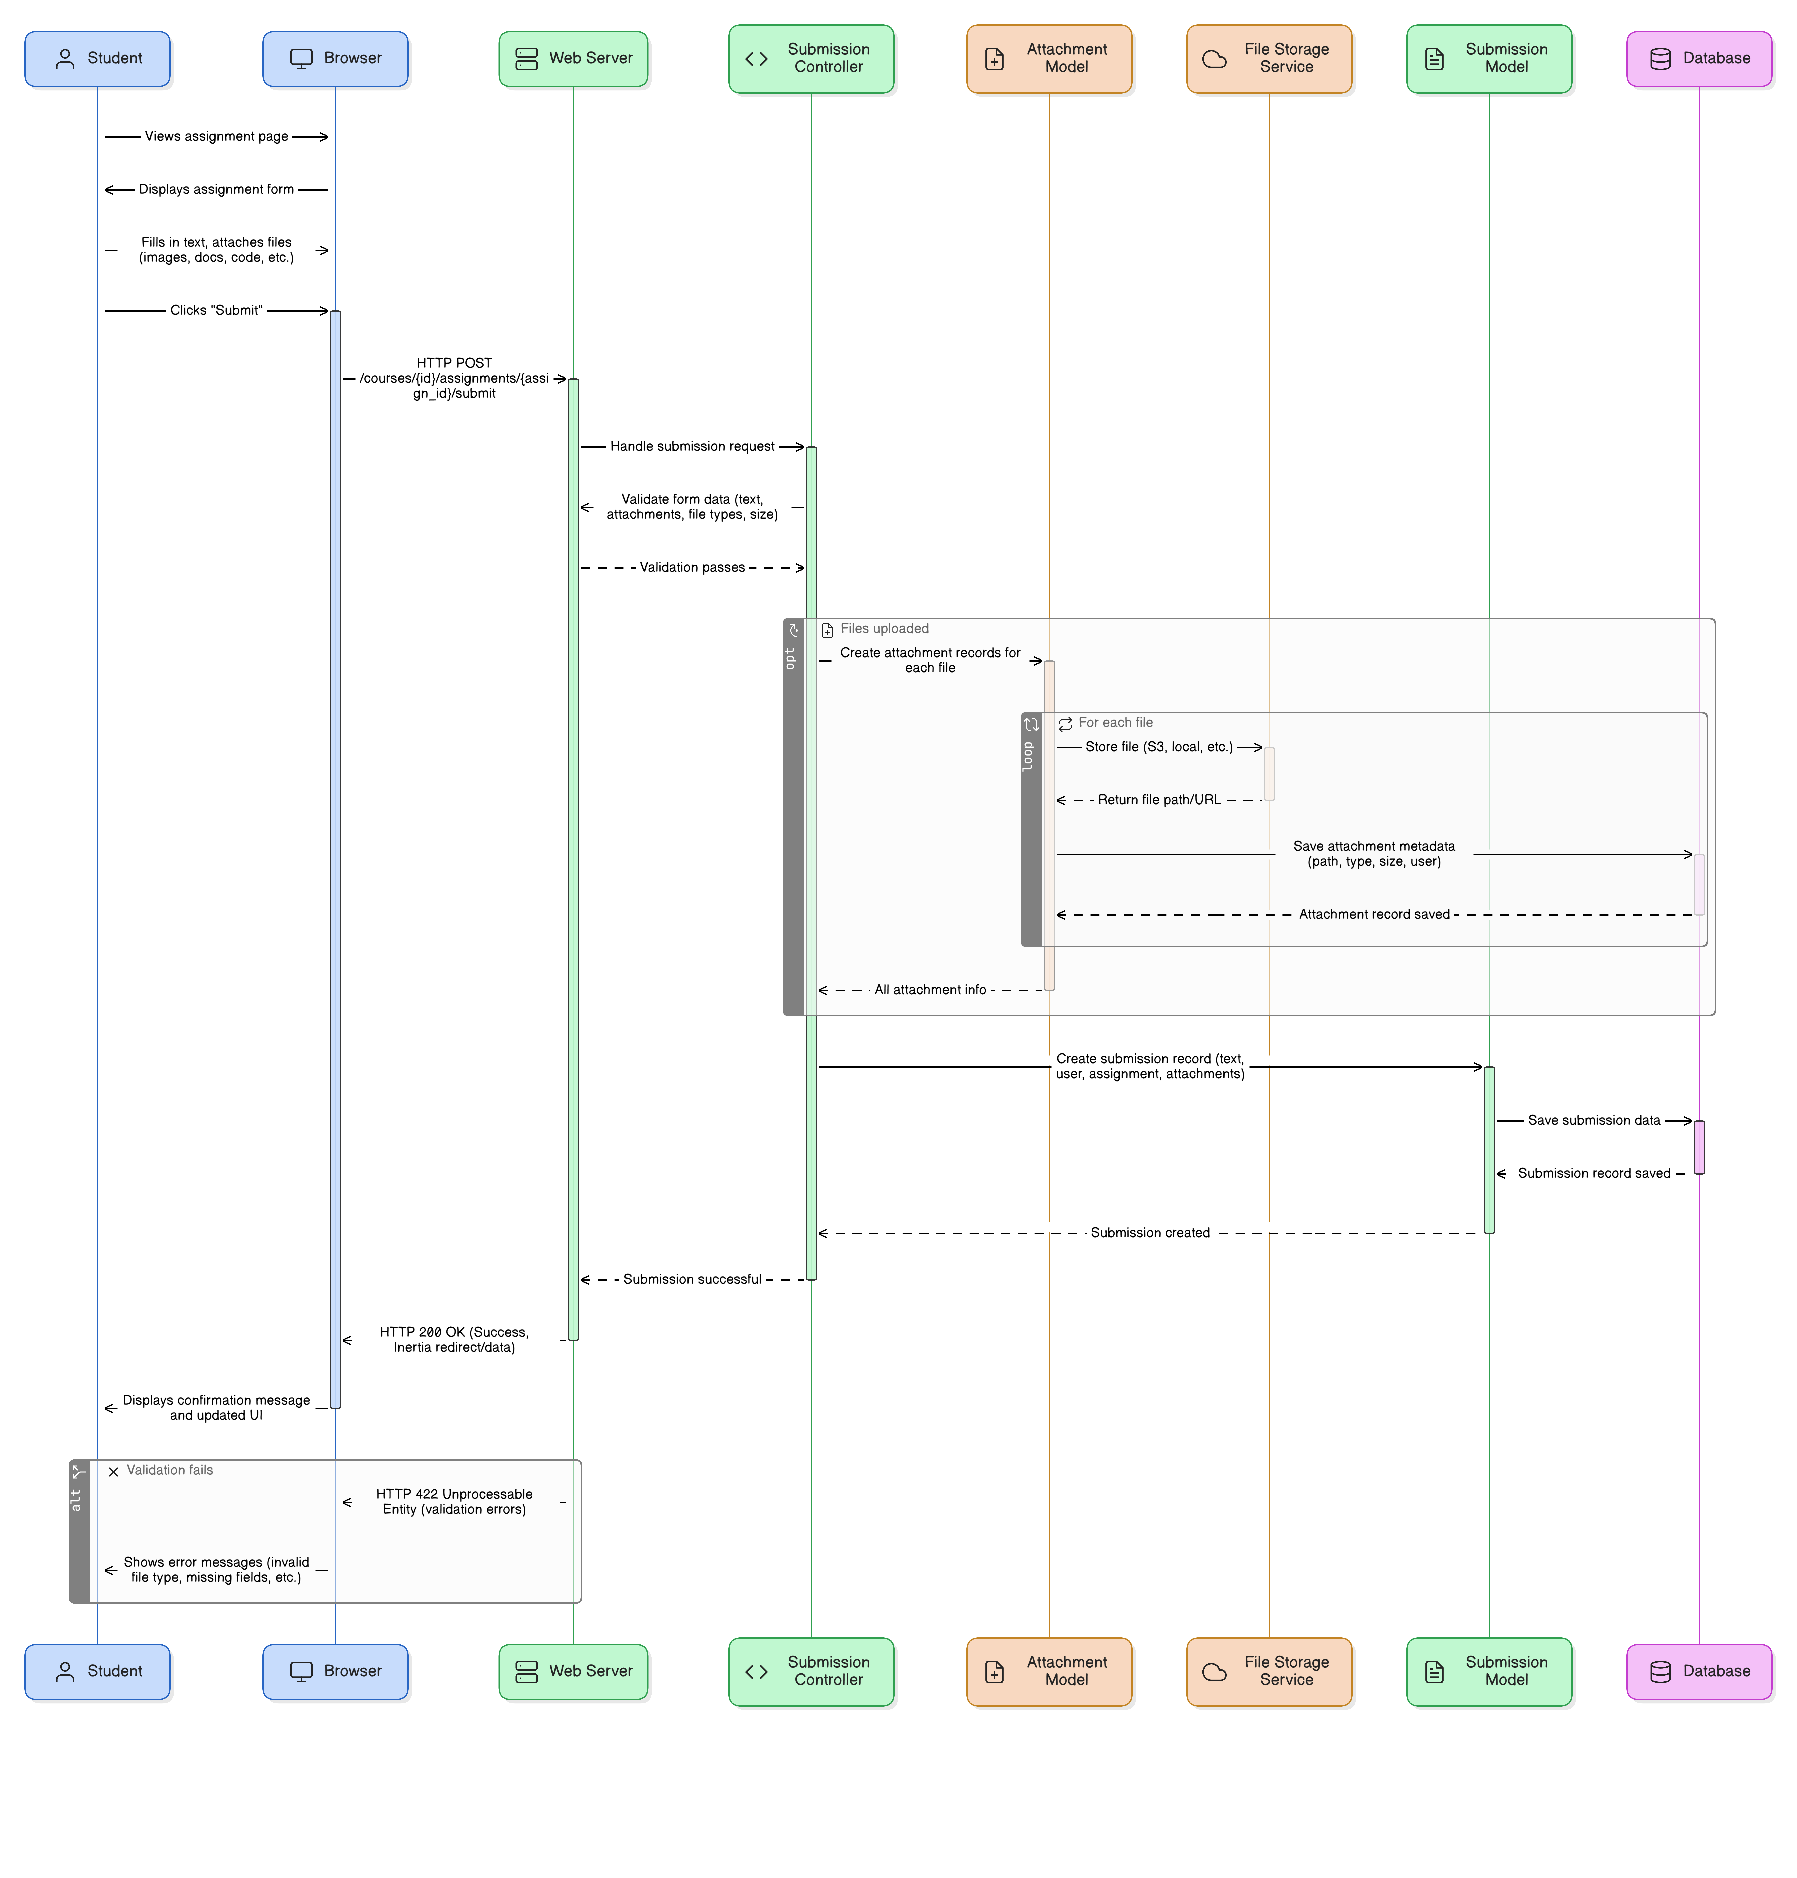
\includegraphics[width=0.9\textwidth]{student-submits-assignment.png}
        \caption{Student Assignment Submission Process - Shows the interaction flow between student, web server, controllers, models, and database when submitting an assignment with file attachments}
        \label{fig:student-submits-assignment}
    \end{figure}
    \FloatBarrier

    \item \textbf{Sequence Diagram: Instructor Grades Submission}
    
    \begin{figure}[!htbp]
        \centering
        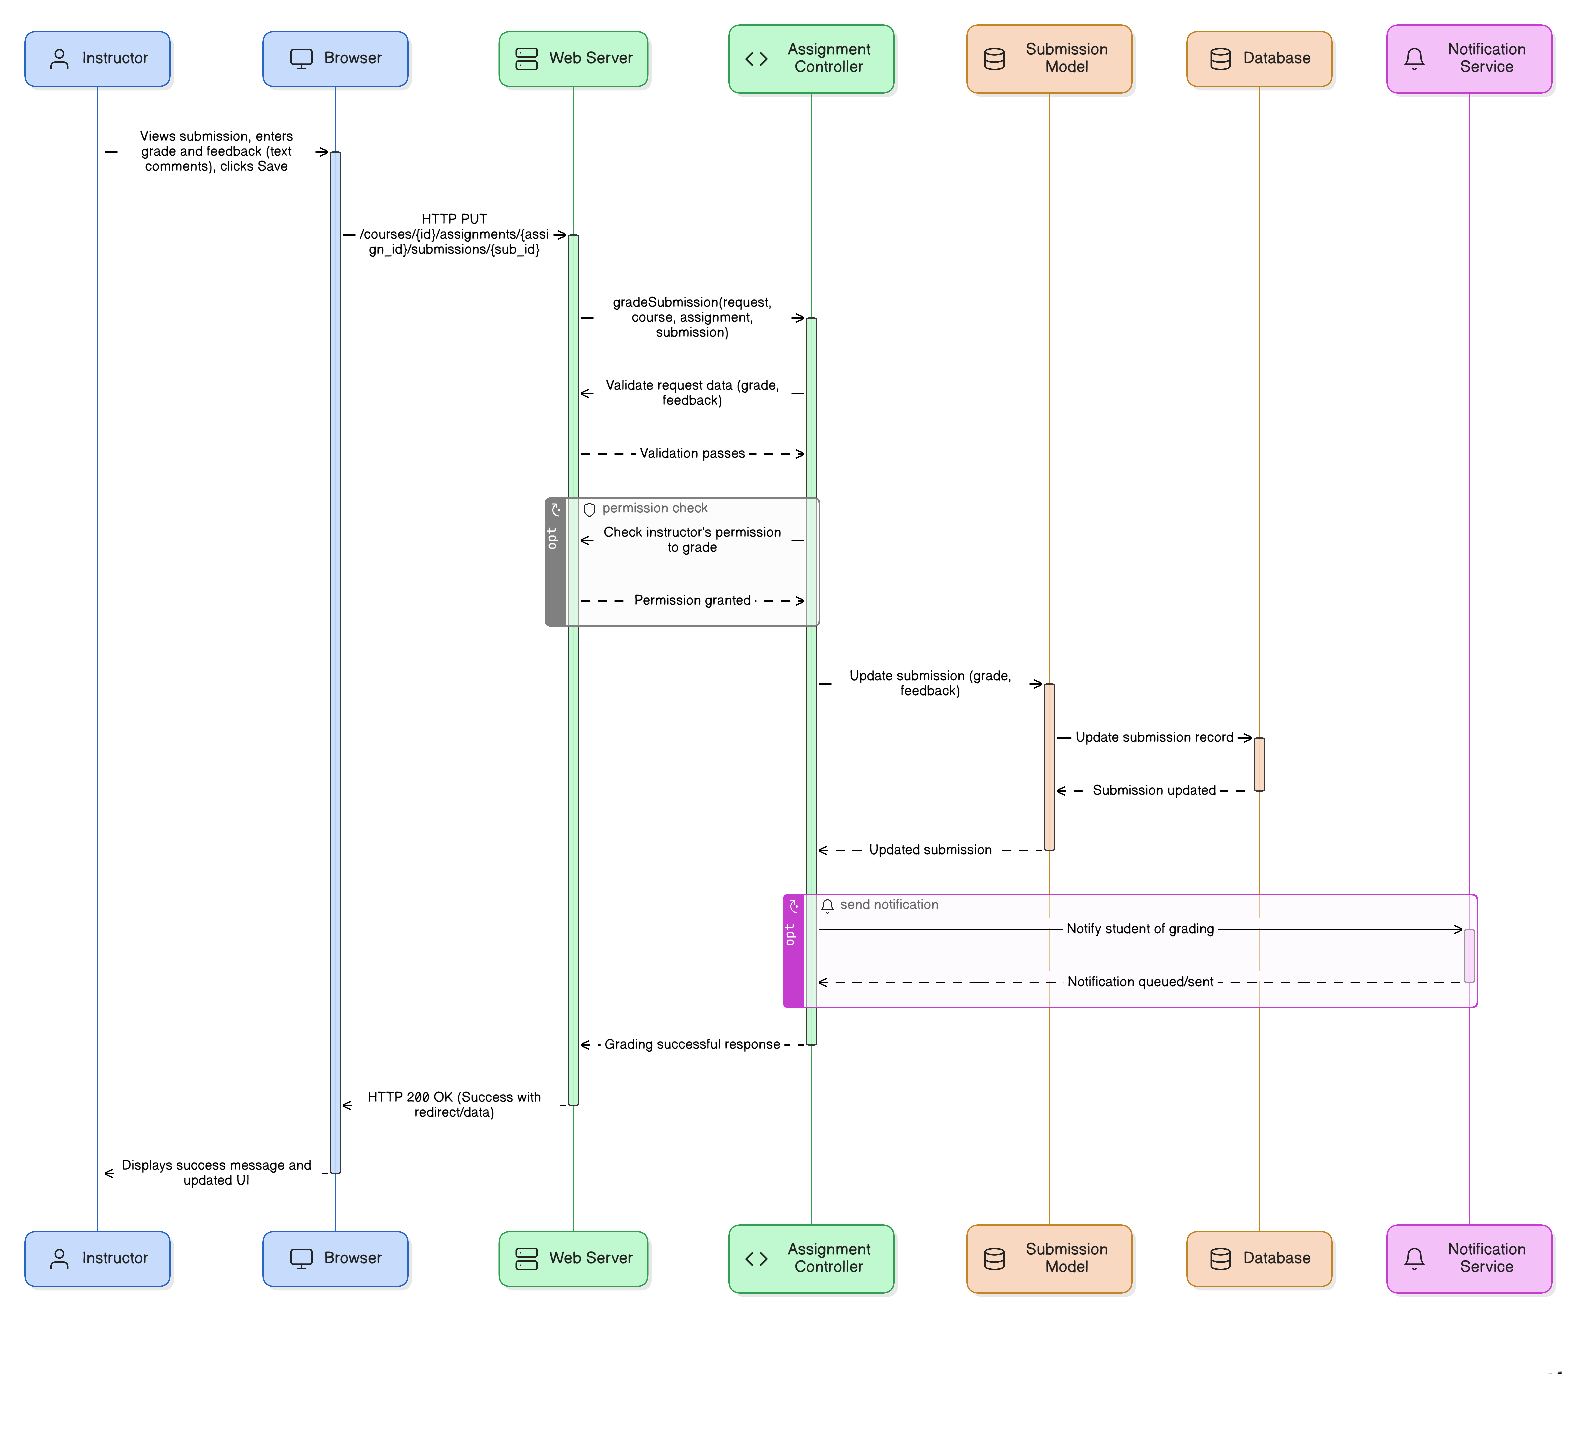
\includegraphics[width=0.9\textwidth]{instructor-grades-submission.png}
        \caption{Instructor Grading Workflow - Demonstrates the process of reviewing student submissions, providing grades and feedback, and updating the database records}
        \label{fig:instructor-grades-submission}
    \end{figure}
    \FloatBarrier

    \item \textbf{Sequence Diagram: User Authentication (Login)}
    
    \begin{figure}[!htbp]
        \centering
        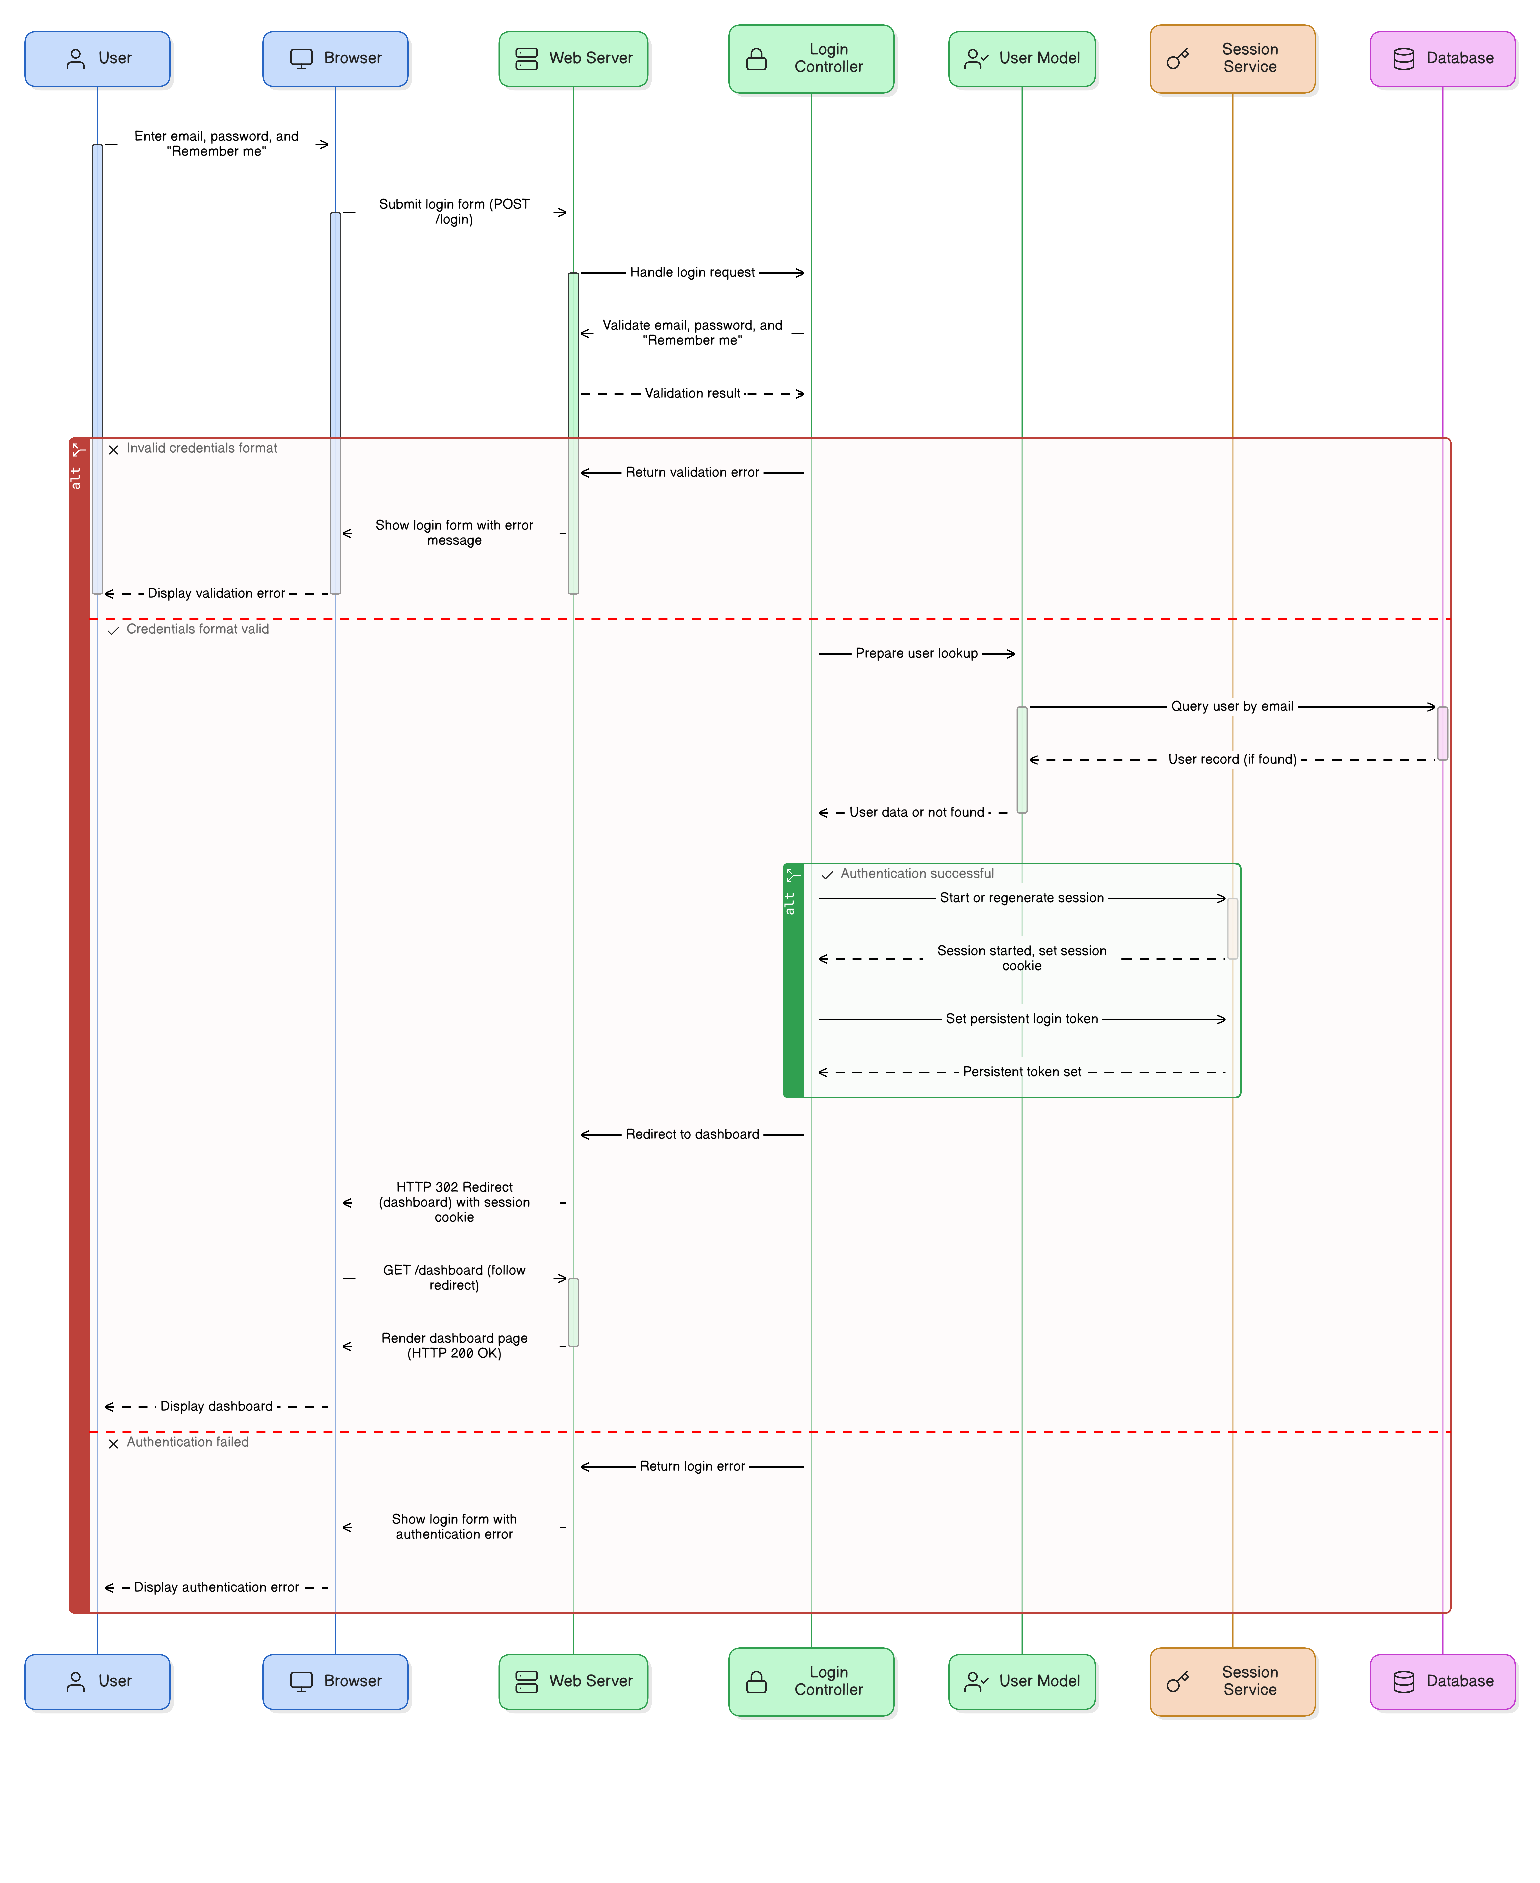
\includegraphics[width=0.9\textwidth]{user-authentication.png}
        \caption{User Authentication Process - Illustrates the login flow including credential validation, session creation, and redirection to the user dashboard}
        \label{fig:user-authentication}
    \end{figure}
    \FloatBarrier
\end{itemize}

\section{Future Development and Enhancement Opportunities}

The current platform establishes a solid foundation for digital education at ENSIASD Taroudant. However, the rapidly evolving landscape of educational technology presents numerous opportunities for expansion and improvement. This section explores potential enhancements that could further strengthen the platform's capabilities and impact:

\subsection{Suggestions for Platform Enhancements/Future Development}

\begin{enumerate}
    \item \textbf{Gamification \& Engagement:}
    \begin{itemize}
        \item Implement a system of points, badges, and certificates awarded for course completions, achieving high scores in quizzes, active participation in discussions, or completing learning streaks.
        \item Introduce course-specific or site-wide leaderboards to foster friendly competition (optional and configurable per course).
        \item Personalized dashboards with visual progress indicators and achievements.
    \end{itemize}
    \item \textbf{Advanced Analytics \& Reporting:}
    \begin{itemize}
        \item \textit{For Students:} Provide more detailed personal dashboards showing time spent on different resources, quiz performance breakdowns by topic, and comparison against anonymized class averages.
        \item \textit{For Instructors:} Offer deeper insights into student engagement (e.g., which resources are most/least accessed), analysis of assignment difficulty, question-level statistics for quizzes, and automated alerts for students at risk of falling behind.
        \item \textit{For Administrators:} Develop comprehensive reports on platform usage (e.g., peak hours, user growth rates), most popular courses, content consumption patterns, and instructor activity.
    \end{itemize}
    \item \textbf{Mobile Application:}
    \begin{itemize}
        \item Develop native (iOS/Android) or hybrid mobile applications to provide students and instructors with convenient on-the-go access.
        \item Features could include offline content access, push notifications for deadlines and announcements, and mobile-optimized interfaces for discussions and submissions.
    \end{itemize}
    \item \textbf{Integrations with External Services:}
    \begin{itemize}
        \item \textbf{Live Virtual Classes:} Integrate with video conferencing tools like Zoom, Google Meet, or BigBlueButton for conducting live lectures, Q\&A sessions, and workshops directly within the platform.
        \item \textbf{Calendar Integration:} Allow users to sync course deadlines, live session schedules, and personal study plans with their Google Calendar, Outlook Calendar, or other calendar applications.
        \item \textbf{Plagiarism Detection:} Integrate with services like Turnitin or Copyscape to check originality of assignment submissions.
        \item \textbf{Single Sign-On (SSO):} Implement SSO with ENSIASD Taroudant's existing institutional identity provider for seamless user authentication.
        \item \textbf{Payment Gateways:} If the platform intends to offer paid courses or certifications in the future, integrate with payment gateways like Stripe or PayPal.
    \end{itemize}
    \item \textbf{Enhanced Accessibility (a11y):}
    \begin{itemize}
        \item Conduct a thorough accessibility audit against WCAG 2.1/2.2 AA or AAA guidelines.
        \item Systematically implement improvements for keyboard navigation, ARIA attributes for dynamic content and custom components, and ensure robust screen reader compatibility.
        \item Offer high contrast themes and user-adjustable font sizes for better readability.
    \end{itemize}
    \item \textbf{Personalized Learning Paths \& AI Features:}
    \begin{itemize}
        \item Develop adaptive learning capabilities where the system suggests or adjusts learning paths based on student performance in quizzes and assignments.
        \item Recommend supplementary resources, remedial exercises, or advanced topics tailored to individual student needs.
        \item Explore AI-powered tutors or Q\&A bots for instant student support.
    \end{itemize}
    \item \textbf{Interactive Content Types \& Authoring:}
    \begin{itemize}
        \item Integrate support for H5P to allow instructors to create rich, interactive HTML5 content directly within the platform.
        \item Enable embedding or importing of SCORM packages for standardized e-learning content.
        \item Develop more sophisticated in-browser coding exercises with automated checks, or specialized simulation tools relevant to ENSIASD's curriculum.
    \end{itemize}
    \item \textbf{Improved Search Functionality:}
    \begin{itemize}
        \item Implement a global search feature allowing users to find content across all their enrolled courses, including resources, discussion posts, announcements, and assignment descriptions.
        \item Introduce more advanced filtering and sorting options within search results (e.g., by date, type, author).
    \end{itemize}
    \item \textbf{Social Learning \& Collaboration Features:}
    \begin{itemize}
        \item Facilitate the creation of study groups or project collaboration spaces within courses, with shared file areas and discussion channels.
        \item Implement a peer review system for assignments, allowing students to provide feedback on each other's work based on defined rubrics.
        \item User profiles could be enhanced with interests, skills, and options to connect with peers.
    \end{itemize}
    \item \textbf{Advanced Certification Module:}
    \begin{itemize}
        \item Develop a robust certification module for automatically generating and issuing digital certificates upon successful course completion.
        \item Ensure certificates are customizable, can include unique verifiable codes or links, and can be easily shared by students (e.g., on LinkedIn).
    \end{itemize}
\end{enumerate}

\subsection{Further Details for the Report Itself}

\begin{enumerate}
    \item \textbf{Deployment Strategy \& Infrastructure:}
    \begin{itemize}
        \item Outline a typical deployment process for a Laravel and React (Inertia.js) application. This could include:
        \begin{itemize}
            \item Server requirements (LEMP/LAMP stack: Linux, Nginx/Apache, MySQL/PostgreSQL, PHP).
            \item Steps: Cloning the Git repository, running \texttt{composer install --no-dev -o}, \texttt{npm install --production}, \texttt{npm run build}.
            \item Configuration: Setting up the \texttt{.env} file with production credentials (database, S3, mail, etc.).
            \item Database: Running migrations (\texttt{php artisan migrate --force}) and initial seeders if necessary.
            \item Queue Workers: Setting up and supervising queue workers (e.g., using Supervisor) for background tasks.
            \item Task Scheduler: Configuring the Laravel scheduler cron job.
            \item Web server configuration for optimal performance and security.
        \end{itemize}
        \item Mention tools like Laravel Forge, Ploi, or a custom CI/CD pipeline (e.g., GitHub Actions, GitLab CI) that could automate and simplify deployment.
    \end{itemize}
    \item \textbf{Security Considerations:}
    \begin{itemize}
        \item Elaborate on Laravel's built-in security features already leveraged:
        \begin{itemize}
            \item CSRF (Cross-Site Request Forgery) protection via tokens.
            \item XSS (Cross-Site Scripting) prevention through Blade's \texttt{\{\{ \}\}} templating (escapes output) and Vue/React's default data binding.
            \item SQL Injection prevention via Eloquent ORM's use of prepared statements.
            \item Secure password hashing (bcrypt by default).
        \end{itemize}
        \item Highlight application-level security measures:
        \begin{itemize}
            \item Input validation using Laravel's Form Requests or validator.
            \item Authorization: Role-based access control (RBAC) via middleware and potentially Laravel Policies or Gates.
            \item Use of HTTPS for all communication.
        \end{itemize}
        \item Recommend ongoing security practices:
        \begin{itemize}
            \item Regularly update dependencies (PHP, Laravel, npm packages).
            \item Security audits and penetration testing.
            \item Secure file upload handling (validation of types, sizes, scanning for malware).
            \item Rate limiting and protection against brute-force attacks.
        \end{itemize}
    \end{itemize}
    \item \textbf{Scalability Aspects:}
    \begin{itemize}
        \item Discuss how the chosen architecture (Laravel/PHP backend) can be scaled:
        \begin{itemize}
            \item \textbf{Horizontal Scaling:} PHP's stateless nature allows for adding more application servers behind a load balancer.
            \item \textbf{Database Scaling:} Strategies like using read replicas for MySQL/PostgreSQL, database sharding (more complex), or choosing scalable cloud database solutions.
            \item \textbf{Caching:} Leveraging Redis (already configured) or Memcached for database queries, sessions, and application data to reduce database load.
            \item \textbf{Background Jobs/Queues:} Offloading time-consuming tasks (e.g., sending notifications, processing large files) to Laravel's queue system.
            \item \textbf{Content Delivery Network (CDN):} Using a CDN to serve static assets (CSS, JS, images) to reduce load on the application server and improve global load times.
            \item \textbf{Optimized Code \& Queries:} Emphasize the importance of efficient code and database query optimization.
        \end{itemize}
    \end{itemize}
    \item \textbf{Project Management Methodology (Suggested):}
    \begin{itemize}
        \item While not directly inferable from the codebase alone, suggest that an Agile methodology (like Scrum or Kanban) would be highly suitable for the development of such a platform.
        \item Benefits: Iterative development, adaptability to changing requirements, regular feedback loops with stakeholders (instructors, students, administrators), and continuous improvement.
    \end{itemize}
    \item \textbf{Contribution Guidelines (for a hypothetical open-source or collaborative future):}
    \begin{itemize}
        \item Briefly mention standard practices if the project were to evolve with community contributions:
        \begin{itemize}
            \item Coding standards (e.g., PSR-12 for PHP, established ESLint/Prettier rules for frontend).
            \item Branching strategy (e.g., Gitflow).
            \item Pull request process (code reviews, automated checks).
            \item Issue tracking and bug reporting guidelines.
            \item Setting up a development environment.
        \end{itemize}
        \item This point is more about future-proofing or if the report context includes open collaboration.
    \end{itemize}
\end{enumerate}

\section{Conclusion}

The ENSIASD E-Learning Platform stands as a testament to thoughtful educational technology design, successfully bridging the gap between traditional academic instruction and modern digital learning requirements. Through its sophisticated integration of Laravel's robust backend capabilities with React's dynamic frontend experience, the platform creates an environment where education technology serves pedagogical goals rather than constraining them.

The platform's architecture demonstrates careful consideration of the diverse stakeholder needs within higher education. Students benefit from intuitive interfaces that prioritize learning over navigation complexity, while instructors gain powerful content creation and assessment tools that enhance rather than complicate their teaching workflows. Administrators receive comprehensive oversight capabilities that maintain institutional standards while supporting academic freedom.

Perhaps most significantly, the platform's technical foundation positions ENSIASD Taroudant for continued innovation in digital education. The modular architecture, contemporary technology stack, and extensible design patterns create numerous opportunities for enhancement and adaptation as educational needs evolve.

This analysis reveals not just a functional e-learning system, but a platform designed for growth, adaptation, and sustained educational impact. The careful balance between current functionality and future flexibility suggests that ENSIASD Taroudant has invested in technology that will continue serving its educational mission for years to come.
\end{document}